% !TEX TS-program = pdflatexmk

\documentclass{AIAA}

\usepackage{algorithm,algpseudocode}
\usepackage{array}
\usepackage{cleveref}
\usepackage{graphicx}
\usepackage[obeyFinal]{todonotes}
\usepackage[caption=false,font=normalsize,labelfont=sf,textfont=sf]{subfig}
\usepackage{url}
\usepackage{diagbox}
\usepackage{multirow}
%\usepackage{bm}
\usepackage[detect-all]{siunitx}


% Define AIAA uses for section and figure references
\Crefname{section}{Sec.}{Sec.}
\Crefname{figure}{Fig.}{Fig.}

% Custom Commands
\newcommand\abs[1]{\left|\,#1\,\right|}
\newcommand{\etal}{\textit{et~al.}}
\newcommand{\eg}{\textit{e.g.}}
\newcommand{\ie}{\textit{i.e.}}
\newcommand{\var}[1]{\textit{#1}} % For use in algorithmic environments
\renewcommand{\arraystretch}{1.3} % Increases spacing between rows in tables

\newcommand{\note}[1]{\todo[inline, author={Kelton}]{#1}}

\newcommand{\toolname}{Critical Phase Analysis Tool}
\newcommand{\toolnameshort}{CPAT}

% declare the path(s) where your graphic files are
\graphicspath{{img/}}
% and their extensions so you won't have to specify these with
% every instance of \includegraphics
\DeclareGraphicsExtensions{.pdf,.jpg,.jpeg,.png}


\begin{document}

\title{Providing Metrics-Based Results to Student Pilots for Critical Phases of General Aviation Flights}

\author{
	Kelton Karboviak\footnote{Graduate Student, Department of Computer Science, 243 Centennial Drive Stop 9015, Grand Forks, ND 58202-9015},
	Travis Desell\footnote{Associate Professor, Department of Computer Science, 243 Centennial Drive Stop 9015, Grand Forks, ND 58202-9015},
	Mark Dusenbury\footnote{Associate Professor, Department of Aviation},
	James Higgins\footnote{Department Chair, Department of Aviation}, and
	Brandon Wild\footnote{Assistant Professor, Department of Aviation}
}
\affiliation{University of North Dakota, Grand Forks, ND 58202, USA}


%----------------------------------------------------------------------------------------
%	ABSTRACT
%----------------------------------------------------------------------------------------

%\abstract{% !TEX root =  ../main.tex

	This work details the development of the \toolname\ (\toolnameshort), a tool for analyzing and grading the quality of approach and landing phases of flight for the National General Aviation Flight Information Database (NGAFID).  General Aviation (GA) accounts for the highest accident rates in Civil Aviation, and the approach and landing phases are when a majority of these accidents occur.  Since GA aircraft typically lack most of the sophisticated technology that exists within Commercial Aviation, detecting phases of flight can be difficult.  Moreover, because of the high variability in GA operations and abilities of the pilot, detecting unsafe flight practices is also not trivial.  This article details the usefulness of an event-driven approach in analyzing the quality and risk level of an approach and landing.  In particular, the application uses several parameters from a flight data recorder (FDR) to detect the phases of flight, detect any safety exceedances during the phases, and assign a metrics-based grade based on the accrued number of risk levels.  The goal of this work is to improve the post-flight debriefing process for student pilots and Certified Flight Instructors (CFIs) by augmenting the currently limited verbal feedback with metrics and visualizations.  By improving the feedback available to students, it is believed that it will help to correct unsafe flying habits quicker, which will also help reduce the GA accident rates in the long-term.  The data was collected from a Garmin G1000 FDR glass cockpit display on a Cessna C172 fleet.  The developed application is able to successfully detect go-arounds, touch-and-goes, and full-stop landings as either stable or unstable with an accuracy of 98.16\%.  The \toolnameshort\ can be used to provide post-flight statistics and user-friendly graphs for educational purposes.  It is capable of assisting both new and experienced pilots for the safety of themselves, their organization, and GA as a whole.}
% !TEX root =  ../main.tex

	This work details the development of the \toolname\ (\toolnameshort), a tool for analyzing and grading the quality of approach and landing phases of flight for the National General Aviation Flight Information Database (NGAFID).  General Aviation (GA) accounts for the highest accident rates in Civil Aviation, and the approach and landing phases are when a majority of these accidents occur.  Since GA aircraft typically lack most of the sophisticated technology that exists within Commercial Aviation, detecting phases of flight can be difficult.  Moreover, because of the high variability in GA operations and abilities of the pilot, detecting unsafe flight practices is also not trivial.  This article details the usefulness of an event-driven approach in analyzing the quality and risk level of an approach and landing.  In particular, the application uses several parameters from a flight data recorder (FDR) to detect the phases of flight, detect any safety exceedances during the phases, and assign a metrics-based grade based on the accrued number of risk levels.  The goal of this work is to improve the post-flight debriefing process for student pilots and Certified Flight Instructors (CFIs) by augmenting the currently limited verbal feedback with metrics and visualizations.  By improving the feedback available to students, it is believed that it will help to correct unsafe flying habits quicker, which will also help reduce the GA accident rates in the long-term.  The data was collected from a Garmin G1000 FDR glass cockpit display on a Cessna C172 fleet.  The developed application is able to successfully detect go-arounds, touch-and-goes, and full-stop landings as either stable or unstable with an accuracy of 98.16\%.  The \toolnameshort\ can be used to provide post-flight statistics and user-friendly graphs for educational purposes.  It is capable of assisting both new and experienced pilots for the safety of themselves, their organization, and GA as a whole.

%\begin{abstract}
%These instructions give you guidelines for preparing papers for AIAA Technical Journals. Use this document as a template if you are using Microsoft Word 2001 or later for Windows, or Word X or later for Mac OS X. Otherwise, use this document as an instruction set. If you previously prepared an AIAA Conference Paper using the Papers Template, you may submit your journal paper in that format with one exception: after you have entered all of your text and figures into the table, be sure to double space your paper before submitting it to WriteTrack$\texttrademark $. Carefully follow the journal paper submission process in Sec. II of this document. Keep in mind that the electronic file you submit will be formatted further at AIAA. This first paragraph is formatted in the abstract style. Abstracts are required \textit{only} for regular, full-length papers. Be sure to define all symbols used in the abstract, and do not cite references in this section. The footnote on the first page should list the Job Title and AIAA Member Grade (if applicable) for each author.
%\end{abstract}

\maketitle


%----------------------------------------------------------------------------------------
%	JOURNAL CONTENT - CHAPTERS
%----------------------------------------------------------------------------------------

% !TEX root =  ../main.tex

\section{Introduction} \label{sec:introduction}

	General Aviation (GA) is one of two branches of Civil Aviation, which pertains to the operation of all non-scheduled and non-military aircraft~\cite{aopa2009what,allen2006general,federal-aviation-administration2016the-economic,kenny201726th}.  GA includes fixed-wing airplanes, helicopters (rotorcraft), balloons, dirigibles, gliders, etc.; and comprises 63\% of all Civil Aviation activity within the U.S.~\cite{aopa2009what,federal-aviation-administration2016the-economic,shetty2012current}.  Performing GA flight analysis is essential for making the GA community safer, as currently GA has the highest accident rates in Civil Aviation~\cite{kenny201726th,aopa-air-safety-institute20172015-2016}.  As of 2014, the total accident and fatality rates for GA fixed-wing aircraft were 5.78 and 1.19 per 100,000 flight hours, respectively; and 75.3\% of GA accidents were caused by pilot-related actions~\cite{kenny201726th}.

	The National General Aviation Flight Information Database (NGAFID) has been developed at the University of North Dakota as a joint university-industry-FAA initiative that is responsible for the curation, dissemination, and analysis of flight data for the General Aviation (GA) sector of Civil Aviation~\cite{clacharlarge-scale,url_ngafid}.  The objective of the NGAFID is to proactively identify accident precursors and mitigate risks associated with unsafe flight practices and aircraft maintenance issues within the GA community.  This is achieved via non-punitive information sharing to educate operators on risks associated with their flights to encourage safer practices~\cite{clacharlarge-scale}.  The analytical tools provided by the NGAFID are free and available to GA pilots who participate by uploading their flight data through the NGAFID web application\footnote{http://www.ngafid.com} or the GAARD mobile application~\cite{url_gaard}.  Subsequently, their flight data is preprocessed and analyzed using various queries.  Many queries are based on threshold criteria called \textit{exceedances}, which are predefined using known limitations of the make/model aircraft or the phase of flight. However, other recent work has focused on developing more advanced analytics through machine learning and other holistic techniques~\cite{sophine2014identifying,sophine2016phd,desell2015evolving,elsaid2016vibration,elsaid2016thesis,desell2014evolving,elsaid2018using}.  Upon logging into the web portal, the user is provided with summaries of any unsafe events (see \Cref{fig:exceedance_example}) and is able to reanimate their flight(s) using X-Plane\footnote{http://www.x-plane.com} or Cesium\footnote{http://www.cesiumjs.org} (see \Cref{fig:cesium_example}).  The intent is to educate participating pilots on any unsafe practices in their flight and maintenance issues with the aircraft which may contribute to an accident/incident. The overall goal of this initiative is to reduce the accident and fatality rates within the GA community.

	\begin{figure}
    	\centering
        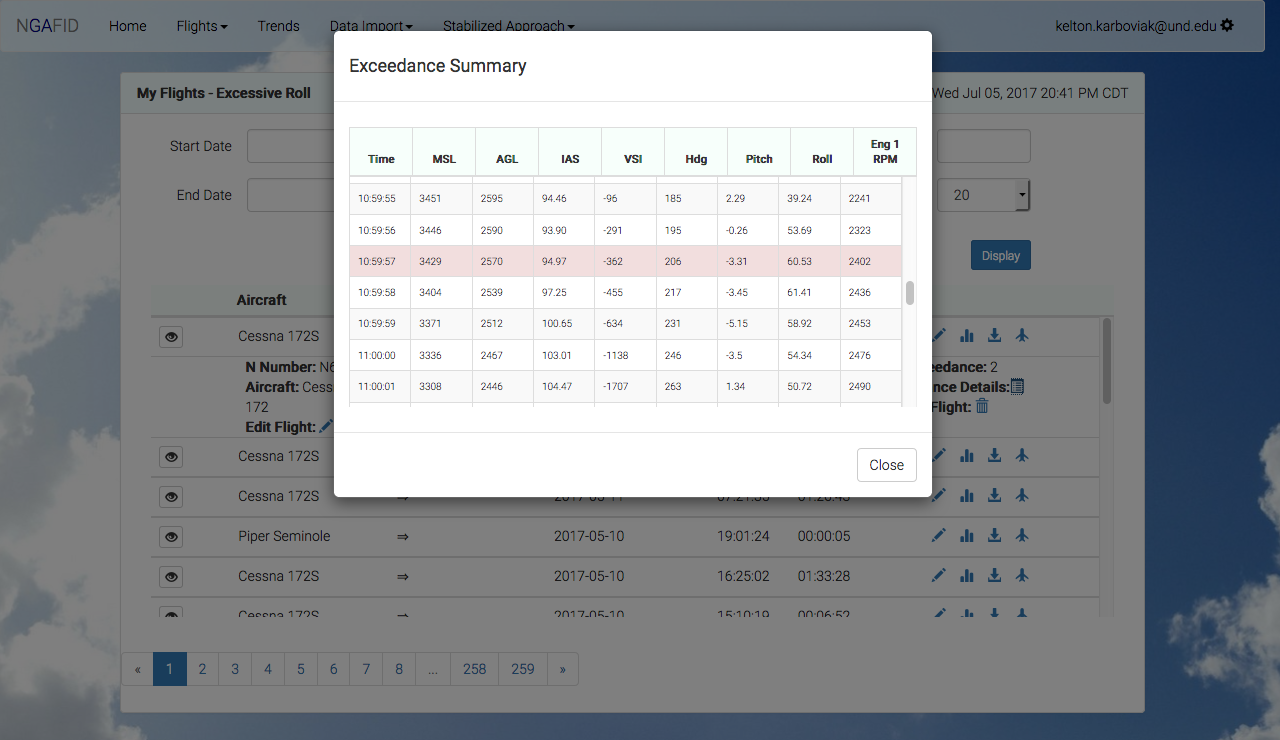
\includegraphics[width=\linewidth]{exceedance_example.png}
        \caption{Screen-shot of a flight which has an excessive roll exceedance.  The exceedance event is highlighted in red.}
        \label{fig:exceedance_example}
    \end{figure}
    
    \begin{figure}
    	\centering
        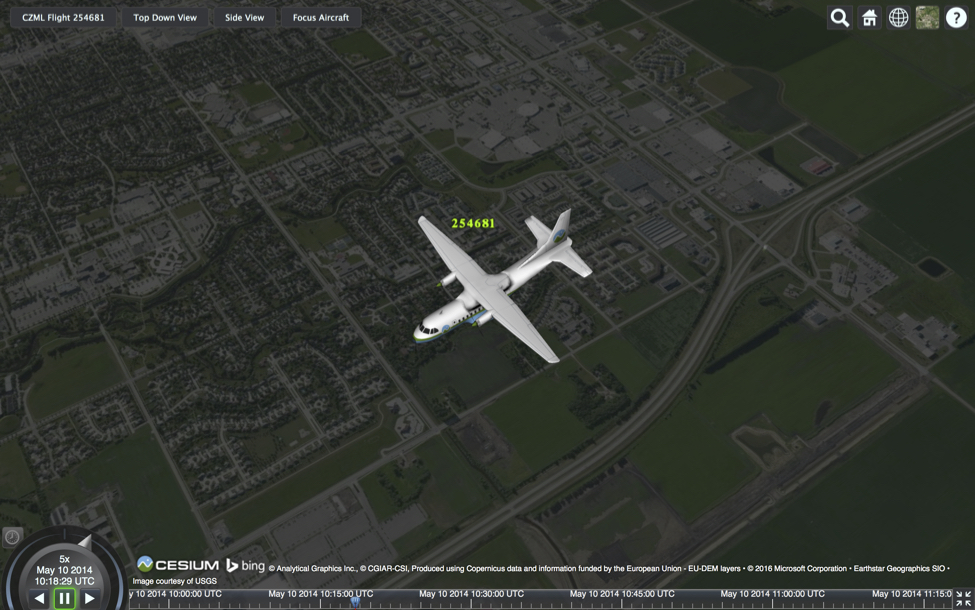
\includegraphics[width=\linewidth]{cesium_example.jpg}
        \caption{Example of in-browser flight reanimation using Cesium.}
        \label{fig:cesium_example}
    \end{figure}


%----------------------------------------
% SCOPE & OBJECTIVES
%----------------------------------------
\subsection{Scope \& Objectives} \label{sec:objectives}

	The goal of this research is to develop an automated grading system, the \toolname\ (\toolnameshort), for analyzing quality of approach and landing phases with a low error rate, reasonable run-time, and that can handle the wide variation of GA flight.  This application will be useful in several different areas:
%
    \begin{itemize}
    	\item provide student pilots with a grade/metric that they can use to gauge a flight's quality, which helps target different student learning techniques,
        \item help improve the flight training process for Certified Flight Instructors (CFI) by making post-flight evaluation more efficient,
        \item help reduce costs of training for the student and institution due to a lesser need for additional training flights, and
        \item help further reduce GA accident and fatality rates.
    \end{itemize}
    

%----------------------------------------
% MOTIVATION
%----------------------------------------
\subsection{Motivation} \label{sec:motivation}

	Despite many safety efforts that have been recently introduced to the GA community, accident rates in the United States remain high.  One way of characterizing flight safety is by identifying \textit{exceedances}, or events that bring the aircraft into an unsafe state dependent on the phase of flight.  By detecting these exceedances, we can identify areas of improvement at the pilot- or organizational-level and additionally educate the pilots on their unsafe practices.  In particular, this research is mainly focused on this aspect of improving teaching feedback for Certified Flight Instructors (CFIs) and student pilots within flight training institutions (although it may be useful to individual private pilots as a side-effect).  Furthermore, the scope of analysis is for the approach and landing phases of flight since these are some of the most critical phases in GA as they ranked \#6 and \#1, respectively, for number of pilot-related accident types in 2014~\cite{kenny201726th}.  These phases present particular challenges in detection of the phase and exceedances due to the high variability in GA operations and flight performance~\cite{goblet2015identifying,goblet2016phase,fala2016detecting}.
    
    At the time of this writing, the feedback that a student pilot receives for their flying performance consists of a verbal debriefing given by the student's CFI.  This process can be prone to errors as both the CFI and student must recall the flight from memory or utilize any notes they were able to take mid-flight.  Additionally, a cross-country flight may last anywhere from 1.5 to 2 hours, which can be a lot to recall after they have landed and returned the aircraft.  This may work well for some students, but not for all as many people do not have a great short-term memory.  For these reasons, an automated system that can provide metrics-based results of their flying performance and allow them to replay their flight will benefit student pilots by providing another means of obtaining feedback, which will cater to students who learn more efficiently with visual materials.


%----------------------------------------
% OUTLINE
%----------------------------------------
\subsection{Outline} \label{sec:outline}

	This research is organized with related works in the areas of aircraft operations, post-flight evaluation tools, NGAFID related work, and data mining techniques in \Cref{sec:related_work}.  \Cref{sec:methodology,sec:implementation} are a continuation of previous work presented in~\cite{karboviak2018classifying}.  The approach to phase of flight identification, exceedance detection, grading, and web interface are discussed in \Cref{sec:methodology}.  The implementation; including the programming languages, libraries, and parallelization techniques used; are discussed in \Cref{sec:implementation}.  Results of the flight analysis are given in \Cref{sec:results}.  Finally, there is a conclusion of the research and a discussion of future work in \Cref{sec:conclusion}.
    
    
    

% !TEX root =  ../main.tex

\section{Related Work} \label{sec:related_work}

%----------------------------------------
% AIRCRAFT OPERATIONS
%----------------------------------------
\subsection{Aircraft Operations}

	In Dr. Ed Wischmeyer's paper, \emph{The Myth of the Unstable Approach}~\cite{wischmeyer2004the-myth}, he discusses how the term ``unstable approach'' is now becoming too vague to be used in accident and incident reports.  He argues there are too many factors that play into an approach; therefore, labeling it solely as an ``unstable approach'' is not sufficient.  This aligns with one of the goals of the \toolname\ in that it was developed to detect unstable approaches and be able to state what the specific parameter was that caused the approach to be unstable.  In doing this, it allows for finer-grained statistics to be generated, which can reveal further patterns to be detected within an organization if it becomes a wide-spread problem.
    
    Nazeri \etal~\cite{Nazeri:2008:Analyzing-Relat} researched accident and incident data from several different commercial flight data sources in order to discover the factors that cause those events.  They created eight high-level categories, each with sub-factors, for classification.  They used an algorithm to analyze the data for correlations between different attribute-value pairs across the accident and incident data sets.  A factor support ratio was calculated for each attribute-value pair and ranked in decreasing order to find the most significant factors.  The following high-level factors were the four top ranked in order:  company, air traffic control, pilot, and aircraft.  They also did a time-series analysis of the data for the ten-year period in which the data was collected (1995-2004).  This time-series data showed the pilot and aircraft factors are generally decreasing over time, while the air traffic control factors are generally increasing.  By uncovering these patterns and analyzing them over time, they were able to find the factors that are leading causes for accidents/incidents and can address these factors for improvement.


%----------------------------------------
% POST-FLIGHT EVALUATION TOOLS
%----------------------------------------
\subsection{Post-Flight Evaluation Tools}

	There are several software projects that have created post-flight evaluation tools, which a pilot can use to analyze their performance during various phases of flight.  Each project has a similar methodology, but varying presentation techniques.  Knighton and Claramunt~\cite{knighton2001an-aeronautical} created a system that included hardware for collecting real-time flight data and an interactive graphical user interface (GUI).  The GUI is capable of 2D flight re-animation and simple plots of the aircraft's vertical profile throughout the flight.  The flight re-animation also has a panel with indicators showing the real-time sensor data at each time step.  They found through experiments, using volunteers, that their interface was intuitive and encouraged exploration of different aspects of flight performance.  Despite the usefulness of the flight parameter graphs, the downside to their research is that any analysis has to be performed manually by the user as there are no automated analysis results provided.
    
    Masiulionis and Stankunas~\cite{masiulionis2017review} provide a review of several software packages for flight analysis including \textit{IGC Flight Replay}, \textit{OziExplorer}, \textit{GPS TrackMaker}, and \textit{ArcGIS}.  They found that none of the packages provided all the aspects they sought:  interactively enabling/disabling map layers, graphing multiple flight parameters on a single plot, and high-resolution maps.  Thus, they experimented with flight analysis and visualization using \textit{Google Earth}.  \textit{Google Earth} met all of their standards, but the only disadvantage is that the altitude and speed graphs can become compressed for flights with an extended duration.  It does not include any features to resize or drill-down into the graphs to make them more viewable.
    
    Goblet \etal~\cite{goblet2016phase,goblet2015identifying} researched into automatically classifying phases of GA flights.  The focus is on the climb, cruise, and descent phases as they are the most difficult phases to identify in GA due to the variation of mission profiles and purposes of flight when compared to Commercial Aviation. Several methods were explored for identifying these phases:  altitude-based and smoothing-and-differentiation-based (which includes down-sampling, moving average, and local regression).  It was found the best method to use for a particular flight is determined by specific characteristics found within that flight.  An algorithm is then given to automatically select the best method for each flight.  Although the climb, cruise, and descent phases are the most difficult to identify, it is known that the approach, landing, and go-around phases are the most critical and dangerous in GA (as discussed in \Cref{sec:introduction}), thus is the reason this work focuses on analysis of those phases. 
    
    Fala and Marais~\cite{fala2016detecting} developed a method of detecting unsafe aircraft parameters, termed ``safety events'', in GA flights.  Similar to phase identification, detecting safety events in GA is difficult due to the variability in operations.  In their research, they only focus on the approach phase and provide the numerical parameter limits for a Cirrus SR20 aircraft during the approach phase.  For each parameter, they provide a Level 1 and Level 2 limit stating that Level 2 is more dangerous than Level 1.  They analyzed the approach phases from a sample of 23 flights using their defined thresholds and performed a one-way ANOVA analysis to evaluate whether the average number of instances for each type of safety event was similar.  They found their initial threshold definitions were not similar enough across the parameters.  They revised the definitions, re-analyzed the flights, and performed another ANOVA analysis to find that they were then significantly similar.  When detecting safety events, Fala and Marais did not distinguish between sporadic exceedances of the thresholds and a span of consecutive exceedances.  This differs from the work in this project, where an event can span multiple seconds instead of only single time steps.
	

%----------------------------------------
% NGAFID RELATED WORK
%----------------------------------------
\subsection{NGAFID Related Work}

	Other work on the NGAFID has focused in two different areas.  In the first, Desell \etal\ have examined methods based on the prediction of flight data parameters using recurrent neural networks (RNNs).  They have shown that training Jordan and Elman RNNs using evolutionary algorithms such as Particle Swarm Optimization and Differential Evolution can provide strong predictive results for flight data parameters such as airspeed, altitude, pitch, and roll~\cite{desell2014evolving}; and that these results can be further refined utilizing a novel neuroevolution technique based on ant colony optimization (ACO) to evolve the structure of the RNNs~\cite{desell2015evolving}.  Further work by ElSaid \etal\ has utilized Long Short-Term Memory (LSTM) RNNs to predict aircraft engine vibration events~\cite{elsaid2016vibration,elsaid2016thesis}.  They later found the structure of the network can be optimized using ACO, which significantly reduces the number of connections required and improves the predictive ability of the RNN~\cite{elsaid2018using}.
    
    The other area has been in utilizing unsupervised machine learning methods to detect anomalous flights.  Clachar \etal\ have used self organizing maps (SOMs), a type of neural network, to both cluster time series flight data and identify anomalous flights~\cite{sophine2014identifying,sophine2016phd} based on approach phases. The SOMs provided significant benefits in terms of parallelism and performance over other clustering methods such as DBSCAN~\cite{ester1996a-density-based}.


%----------------------------------------
% DATA MINING TECHNIQUES
%----------------------------------------
\subsection{Data Mining Techniques}

	Harris \etal~\cite{harris-jr.1998recent} of MITRE Corporation mined accident and incident reports provided by the International Civil Aviation Organization (ICAO) in order to determine the specific attributes that were the cause in each kind of report and also needed to be considered ``interesting'' (i.e., anything that is an exception to commonly accepted knowledge among aviation experts) by the aviation expert who collaborated with them.  They discovered that using traditional data mining methods was not sufficient enough to find ``interesting'' results.  This is because experts have studied the field of aviation so extensively that all the obvious rules and correlations have already been discovered.  Next, they developed their own system called Smithers, which uses a technique called attribute focusing, that finally uncovered an interesting correlation which shows that having an advanced heads up display (HUD) can help reduce the amount of damage as a result of a runway incursion\footnote{Defined by the Federal Aviation Administration (FAA) as, ``any occurrence at an aerodome involving the incorrect presence of an aircraft, vehicle, or person on the protected area of a surface designated for the landing and take off of aircraft''~\cite{federal-aviation-administrationrunway}.}.  This shows that even though aviation safety has been studied extensively, there are still new correlations that can be made when applying several different data mining methods.
    
    Matthews \etal~\cite{matthews2013discovering} performed similar research in which their goal was to find anomalous data in flights.  They differ in the fact that they used algorithms that could analyze at both a fleet-level and flight-level.  Doing this allowed them to find anomalies for an entire organization or just a single flight, which makes it very useful in order to find patterns of problems.  This idea is similar to the NGAFID project in which flight data can be analyzed on multiple levels while giving statistics for each.

% !TEX root =  ../main.tex

\section{Methodology} \label{sec:methodology}

	The \toolname\ provides several features: \textit{(i)} phase of flight identification, \textit{(ii)} quality analysis of each phase, \textit{(iii)} grade assignment, and \textit{(iv)} a web interface to display results.  Since there are three separate phases of concern, there will be a separate subsection for each in both identification and quality analysis.  These features are discussed in more detail in the rest of this Chapter.

%----------------------------------------
% PHASE IDENTIFICATION
%----------------------------------------
\subsection{Phase of Flight Identification} \label{sec:phase_identification}

	%----------
    % APPROACH
    %----------
	\subsubsection{Approach}
    
    	The approach phase is defined as the time between the aircraft entering the airport's traffic pattern (shown in \Cref{fig:traffic_pattern}), or 1,000 feet above the runway elevation, to the beginning of the landing flare under Visual Flight Rules (VFR).  For Instrument Flight Rules (IFR), it is the time from the Initial Approach Fix (IAF) to the beginning of the landing flare~\cite{cictt2013phase}.
        
        \begin{figure}
        	\centering
            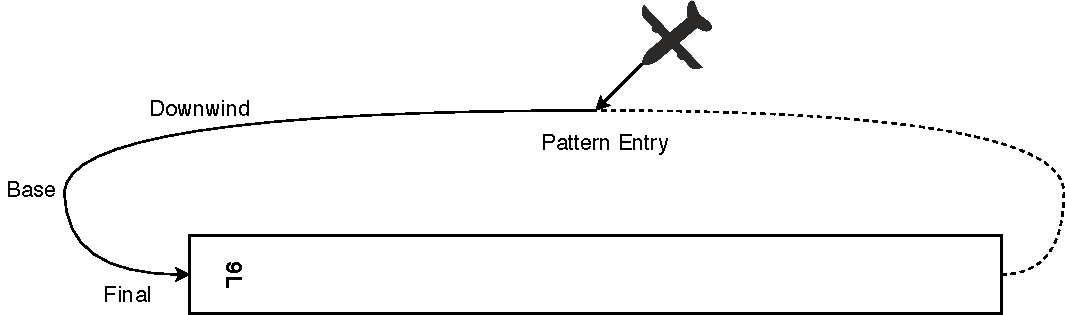
\includegraphics[width=\linewidth]{img/airport_traffic_pattern}
            \caption{Example showing an airport's traffic pattern and the subphases of the approach.}
            \label{fig:traffic_pattern}
        \end{figure}
        
        Along with detecting the approach phase (\Cref{alg:detect_approach}), this section also details the algorithms for detecting \textit{(i)} the airport and runway that the aircraft is approaching and \textit{(ii)} the final turn so it can later be analyzed for an undershoot or overshoot.
        
        The algorithm for detecting an aircraft's approach needs to iterate through all of the time values since there can be multiple approaches within a single flight.  Once the algorithm detects the aircraft is 1 mile away from an airport and is less than 500 feet above ground level (AGL) (\Cref{alg:detect_approach} Line 6), it is determined that the pilot is beginning an approach and a unique approach identifier is generated in order to store metadata later in the process.  Next, the algorithm continues to iterate through time values until either the aircraft goes under 200 ft AGL, or it goes back above 500 ft AGL, which will then be recorded as a go-around later in the process (\Cref{alg:detect_approach} Lines 8-12).  If the aircraft goes under 200 ft AGL, then it is determined to be on the final approach.  The aircraft is considered to be on the final approach while it is within 1 mile away from the airport and it is between 50 and 200 feet AGL inclusive (\Cref{alg:detect_approach} Lines 16-22).
    
    Once the aircraft either goes above 200 feet AGL or goes below 50 feet AGL, then the final approach is marked as finished, and the critical metadata associated with the approach is stored.  At this point, the runway that is being approached can be detected using a combination of the aircraft's current geolocation and heading since the intended runway may not be closest to the aircraft depending on the degree of the final turn (\Cref{alg:detect_approach} Line 24).
        
        %%%%% Detect Approaches Pseudo-code
        \begin{algorithm}
            \begin{algorithmic}[1]\raggedright
            	\State $ \var{airplanePoint} \gets \var{data[i].geoPoint} $
            	\State $ \var{airport} \gets \var{detectAirport(airplanePoint)} $
                \State $ \var{airplaneAltitude} \gets \var{data[i].altitude} $
                \State $ \var{heightAGL} \gets \var{airplaneAltitude} - \var{airport.altitude} $
                \State $ \var{distance} \gets \var{airplanePoint.distanceTo(airport.geoPoint)} $
                \If{$ \var{distance} < 1$\,mi and $\var{heightAGL} < 500$\,ft}
                    \State $ \var{apprID} \gets \var{genNewApproachID()} $
                    \While{$ 200\,\text{ft} < \var{heightAGL} < 500\,\text{ft} $ and $ \var{i} < \var{data.length} $}
                        \State $ \var{airplaneAltitude} \gets \var{data[i].altitude} $
                        \State \var{heightAGL} $ \gets $ \var{airplaneAltitude} $-$ \var{airport.altitude}
                        \State $ i \gets i + 1 $
                    \EndWhile

                    \State $ \var{approachStartTime} \gets i $
                    \State $ \var{airplaneHdg} \gets \var{data[i].hdg} $
                    \State $ \var{airplanePoint} \gets \var{data[i].geoPoint} $

                    \While{$ \var{distance} < 1$\,mi and $ 50\,\text{ft} \leq \var{heightAGL} \leq 200\,\text{ft} $ and $ \var{i} < \var{data.length} $}
                        \State $ \var{airplaneAltitude} \gets \var{data[i].altitude} $
                        \State $ \var{airplanePoint} \gets \var{data[i].geoPoint} $
                        \State $ \var{distance} \gets \var{airplanePoint.distanceTo(airport.geoPoint)} $
                        \State $ \var{heightAGL} \gets \var{airplaneAltitude} - \var{airport.altitude} $
                        \State $ i \gets i + 1 $
                    \EndWhile

                    \State $ \var{approachEndTime} \gets i $
                    \State $ \var{runway} \gets $ \var{detectRunway(airplanePoint, airplaneHdg, airport)}
                    \State \var{approaches[apprID]} $ \gets $ store approach metadata
                    \State \Return \var{(approachStartTime, approachEndTime)}
                \EndIf
            \end{algorithmic}
            \caption{Pseudo-code for function which detects when an aircraft is approaching a runway.}
            \label{alg:detect_approach}
        \end{algorithm}
        
        
        %----------
        % AIRPORT DETECTION
        %----------
        \paragraph{Airport Detection} \label{sec:detect_airport}
        
        	For identifying the airport that is being approached, a QuadTree~\cite{finkel1974quad} data structure was used.  It was used due to the fact that a two-dimensional tree structure is needed in order to efficiently find the closest airport latitude and longitude point when given the aircraft's latitude and longitude.  The QuadTree is constructed using a list of airport objects from a database then is optimized.  Both the insertion and searching algorithms yield $\mathcal{O}(\log n)$ complexity.


        %----------
        % RUNWAY DETECTION
        %----------
        \paragraph{Runway Detection}
        
            The algorithm used for finding the runway that is being approached is a simple sequential search with a constraint that the difference between the aircraft's heading and the runway's heading must be within an upper limit.  The reasoning for this constraint is the fact that the runway closest to the aircraft may not necessarily be the one it is approaching depending on the arrangement of the runways and the degree of the final turn (see \Cref{fig:runway_selection}).  A value of $20^\circ$ was used for the heading constraint since it is double the value used for detecting a heading exceedance (see \Cref{tab:approach_thresholds}).  Thus if the runway returned by the algorithm is not the intended runway, it means the aircraft's heading is significantly off-center from the runway's heading and the pilot will need to perform severe corrections to get back on course.
            
            In this case, using a sequential search is efficient enough since an airport has a very small number of runways, whereas there are thousands of airports within the United States which requires a more sophisticated algorithm.  The runway detection algorithm is given in \Cref{alg:detect_runway}.
            
            
            \begin{figure}
            	\centering
				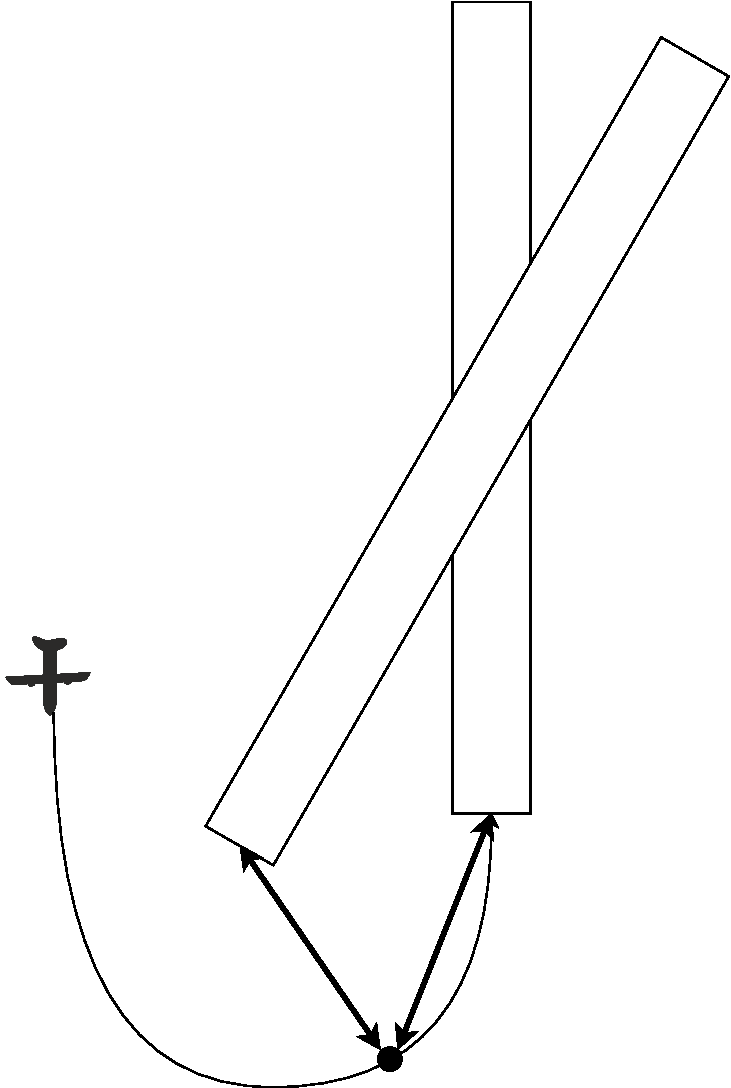
\includegraphics[width=0.5\linewidth]{runway_selection_example}
				\caption{Example showing that the closest runway to the aircraft may not necessarily be the one they are attempting to land on.  If we use the black dot as a reference point for when we attempt to detect the runway, it can be seen that the runway on the left may actually be closer.  However, the aircraft's heading will match closer to the runway on the right (the pilot's intended target).  This is the purpose of searching for the closest runway with a constraint on the heading difference.}
				\label{fig:runway_selection}
            \end{figure}
            

            %%%%% Detect Runway Pseudo-code
            \begin{algorithm}
                \begin{algorithmic}[1]\raggedright
                    \Function{DetectRunway}{airplanePoint, airplaneHdg, airport}
                        \State $ \var{theRunway} \gets \textit{NULL} $
                        \State $ \var{closestDistance} \gets \infty $

                        \For{\var{runway} in \var{airport.runways}}
                            \If{$ \abs{\var{headingDifference(runway.hdg, airplaneHdg)}} \leq 20^\circ $}
                                \State $ \var{distance} \gets \var{airplanePoint.distanceTo(runway.geoPoint)} $
                                \If{$ \var{distance} \le \var{closestDistance} $}
                                    \State $ \var{theRunway} \gets \var{runway} $
                                    \State $ \var{closestDifference} \gets \var{difference} $
                                \EndIf
                            \EndIf
                        \EndFor

                        \State \Return{theRunway}
                    \EndFunction
                \end{algorithmic}
                \caption{Pseudo-code for \textit{detectRunway} function which detects the runway an aircraft is approaching.}
                \label{alg:detect_runway}
            \end{algorithm}
        
        
        %----------
        % FINAL TURN DETECTION
        %----------
        \paragraph{Final Turn Detection}
        
        	In order to detect the final turn subphase of the approach, we first get the previous three minutes of data before the approach ends.  The previous three minutes are used to reduce the search space and because it does not make logical sense for a final turn to occur greater than three minutes before the approach ends.  Next, the algorithm searches for the final turn start and end time.  It finds these by searching for the points at which the aircraft's heading creates a $90^\circ$ and $15^\circ$ angle, respectively, to the runway's heading.  A visualization of these reference points can be seen in \Cref{fig:final_turn_example}.  The search is performed backwards through the slice of data in order to obtain the last occurrence of each angle difference.  Once both points have been found, they are stored for later use in the analysis stage.  If the aircraft did not have a heading difference greater than $90^\circ$ in the final three minutes, the pilot performed a straight-in approach and, consequently, did not execute the final turn subphase.
        	The final turn detection algorithm is given in \Cref{fig:detect_final_turn}.
            
            \begin{figure}
            	\centering
                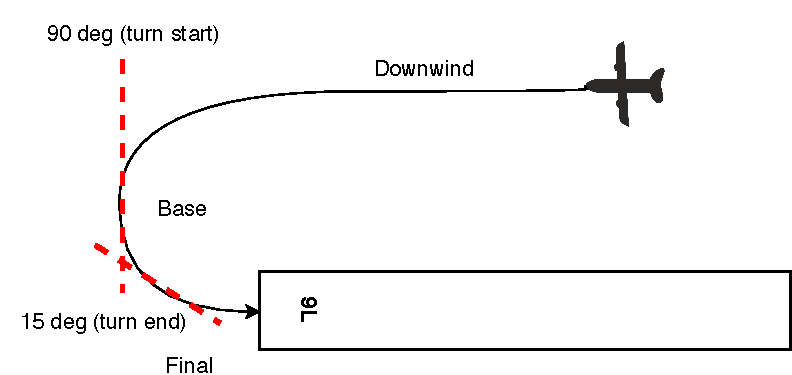
\includegraphics[width=\linewidth]{turn_to_final}
                \caption{Example showing the approach subphases and the slice of data used in the final turn analysis.  The dashed lines represent when the final turn starts ($90^\circ$ heading difference) and ends ($15^\circ$ heading difference).}
                \label{fig:final_turn_example}
            \end{figure}
        
            %%%%% Detect Final Turn Pseudo-code
            \begin{algorithm}
                \begin{algorithmic}[1]\raggedright
                    \Function{DetectFinalTurn}{approachEndTime, runway}
                        \State $ \var{last3Mins} \gets $ get previous 3 mins of data before \var{approachEndTime}
                        \State $ \var{turnStartTime} \gets \textit{NULL} $
                        \State $ \var{turnStartFound} \gets \textit{false} $
                        \State $ \var{turnEndTime} \gets \textit{NULL} $
                        \State $ \var{turnEndFound} \gets \textit{false} $
                        \State $ \var{i} \gets \var{last3Mins.length} - 1 $
                        
                        \Comment Loop backwards through the last 3 mins of data
                        \While{not \var{turnStartFound} and not \var{turnEndFound} and $\var{i} \geq 0$}
                        	\State $ \var{headingError} \gets \abs{\var{headingDifference(runway.hdg, last3Mins[i].hdg)}} $
                            \If{$\var{headingError} \geq 90$ and not \var{turnStartFound}}
                            	\State $ \var{turnStartTime} \gets \var{i} $
                                \State $ \var{turnStartFound} \gets \textit{true} $
                            \EndIf
                            \If{$\var{headingError} \geq 15$ and not \var{turnEndFound}}
                            	\State $ \var{turnEndTime} \gets \var{i} $
                                \State $ \var{turnEndFound} \gets \textit{true} $
                            \EndIf
                            
                            \State $ \var{i} \gets \var{i} - 1 $
                        \EndWhile
                        
                        \State $ \var{approaches[apprID]} \gets $ store final turn metadata
                        \State \Return \var{(turnStartTime, turnEndTime)}
                    \EndFunction
                \end{algorithmic}
                \caption{Pseudo-code for function which detects the final turn subphase of the approach.}
                \label{fig:detect_final_turn}
            \end{algorithm}
        
        
    
    %----------
    % LANDING
    %----------
    \subsubsection{Landing}
    
    The landing phase is defined as the time from the beginning of the landing flare until the aircraft performs one of the following actions: \textit{(i)} exits the landing runway, \textit{(ii)} comes to a complete stop on the runway (full-stop), or \textit{(iii)} when power is applied for takeoff in the case of a touch-and-go landing~\cite{cictt2013phase}.
    
    The landing phase and result detection is able to differentiate between a full-stop, touch-and-go, and a go-around\footnote{Go-around is included here as a possibility for the result of a landing phase since only one of the full-stop, touch-and-go, and go-around maneuvers can be executed after an approach/landing even though the aircraft does not physically contact the ground.}.  Pseudo-code for this process is given in \Cref{alg:detect_landing}.
    
    This detection algorithm iterates through time values starting where the final approach detection finished (\Cref{alg:detect_landing} Lines 10-29).  It continues to iterate while the aircraft is below 500 feet AGL; or if it is the aircraft's final landing and the time values run out, then it stops analyzing.  While the algorithm iterates through the time values, it checks if the aircraft's indicated airspeed (IAS) is less than or equal to 35 knots (\Cref{alg:detect_landing} Line 13).  If this is true, then it is determined the aircraft is no longer traveling at a flying speed, thus it is making a complete stop.  The stall speed of a Cessna 172S aircraft is 40 knots IAS (KIAS)~\cite{und_poh}; therefore, the value of 35 knots guarantees the aircraft cannot be flying.  In order to detect a touch-and-go landing, the previous five elevation readings are stored and their average is calculated (\Cref{alg:detect_landing} Lines 20-28).  If it is found the aircraft is not making a stop-and-go landing, then the average elevation for the last five seconds is checked to see if it is less than five feet AGL (\Cref{alg:detect_landing} Line 15).  This means the aircraft is still at a flying speed (above 35 knots) and is also maintaining a stable elevation of five feet or less for at least five seconds.
    
    Once the aircraft goes above 500 feet AGL or the time values run out, then the landing result is determined from the conditions found during the analysis (\Cref{alg:detect_landing} Line 32 and \Cref{alg:landing_result_helper}).  If it was found the aircraft was making a complete stop, then a value of ``full-stop'' is stored.  If it was not making a complete stop and had a relatively stable elevation of 5 feet or less above the runway, then a value of ``touch-and-go'' is stored.  The final result type, ``go-around'', is used as a fall-through since there are only three classifications, as mentioned previously.  The three landing result types and how they are detected are summarized in \Cref{tab:landing_types}.
    
    After the landing is classified, then it is determined whether there is a takeoff phase that follows the current landing phase.  If the end of the data has been reached or a go-around is being performed (\Cref{alg:detect_landing} Line 33), there will not be a subsequent takeoff phase.  Otherwise, we need to find the transition from landing to takeoff.  This is done by finding the index of the engine's minimum RPM value between \textit{landingStartTime} and \textit{landingEndTime} (\Cref{alg:detect_landing} Line 36 and \Cref{alg:last_rpm_helper}).  By using the engine's minimum RPM value, we know all RPM values afterwards will be greater, which means the pilot will be using more throttle in order to takeoff.  The \textit{landingEndTime} is then reset to this transition mark.  Lastly, the critical metadata found during the analysis is stored.
    
    %%%%% Detect Landing Pseudo-code
   	\begin{algorithm}
    	\begin{algorithmic}[1]
        \Function{DetectLanding}{approachEndTime, runway}
        	\State $ \var{landingStartTime} \gets \var{approachEndTime} $
        	\State $ \var{i} \gets \var{approachEndTime} $
        	\State $ \var{airplaneAltitude} \gets \var{data[i].altitude} $
            \State $ \var{heightAGL} \gets \var{airplaneAltitude} - \var{runway.altitude} $
            
            \State $ \var{isFullStop} \gets \textit{false} $
            \State $ \var{isTouchAndGo} \gets \textit{false} $
            \State $ \var{elevations} \gets \var{[]}$
            \State $ \var{avg5SecElevation} \gets 5\,\text{ft} + 1 $
            	\Comment value to guarantee first check passes
            
            \While{$\var{heightAGL} < 500$\,ft and $\var{i} < \var{data.length}$}
            	\If{not \var{isFullStop}}
                	\State $ \var{airplaneIAS} \gets \var{data[i].ias} $
                    \If{$ \var{airplaneIAS} \leq 35$\,kts}
                    	\State $ \var{isFullStop} \gets \textit{true} $
                    \ElsIf{$ \var{avg5SecElevation} \leq 5$\,ft}
                    	\State $ \var{isTouchAndGo} \gets \textit{true} $
                    \EndIf
                \EndIf
                \State $ i \gets i + 1 $
                \State $ \var{airplaneAltitude} \gets \var{data[i].altitude} $
                \State $ \var{heightAGL} \gets \var{airplaneAltitude} - \var{runway.altitude} $
                \If{$ \var{elevations.length} < 5$\,seconds}
                	\State $ \var{elevations.append(heightAGL)} $
                \Else
                	\State $ \var{elevations.pop()} $
                    \State $ \var{elevations.append(heightAGL)} $
                    \State $ \var{avg5SecElevation} \gets \var{avg(elevations)} $
                \EndIf
            \EndWhile
            
            \State $ \var{landingEndTime} \gets \var{i} $
            \State $ \var{isEndOfData} \gets \var{landingEndTime} == \var{data.length} - 1 $
            
            \State $ \var{landingResult} \gets \var{getLandingResult(isFullStop, isTouchAndGo)} $
         
            \State $ \var{isFollowedByTakeoff} \gets not (\var{isEndOfData} $ or $ \var{landingType} == \text{`go-around'}) $
            
            \Comment{If landing is followed by a takeoff, then we need to find the transition from landing to takeoff}
            \If{\var{isFollowedByTakeoff}}
            	\State $ \var{landingDataSlice} \gets $ get slice of data between \var{landingStartTime} and \var{landingEndTime}
                
                \Comment{Marks where the pilot is transitioning from landing to takeoff}
            	\State $ \var{lastOccurrence} \gets \var{getLastOccurrenceOfMinRPM(landingDataSlice)} $
                \State $ \var{landingEndTime} \gets \var{lastOccurrence} $
            \EndIf
            
            \State $ \var{approaches[apprID]} \gets $ store landing metadata
            \State \Return \var{(landingStartTime, landingEndTime)}
        \EndFunction
        \end{algorithmic}
        \caption{Pseudo-code for function which detects the landing from its associated approach.}
        \label{alg:detect_landing}
    \end{algorithm}
    
    
    \begin{algorithm}
    	\begin{algorithmic}[1]
        	\Function{GetLandingResult}{isFullStop, isTouchAndGo}
        		\If{\var{isFullStop}}
                    \State $ \var{landingResult} \gets $ `full-stop'
                \ElsIf{\var{isTouchAndGo}}
                    \State $ \var{landingResult} \gets $ `touch-and-go'
                \Else
                    \State $ \var{landingResult} \gets $ `go-around'
                \EndIf
                \State \Return \var{landingResult}
            \EndFunction
        \end{algorithmic}
        \caption{Pseudo-code for \var{getLandingResult} helper function.}
        \label{alg:landing_result_helper}
    \end{algorithm}
    
    
    \begin{algorithm}
    	\begin{algorithmic}[1]
        	\Function{GetLastOccurrenceOfMinRPM}{dataSlice}
        		\State $ \var{minRPM} \gets \var{min(dataSlice[`rpm'])} $
                \State $ \var{lastOccurrence} \gets 0 $
                \State $ \var{i} \gets 0 $
                
                \While{$\var{i} < \var{dataSlice.length}$} \Comment{loop through slice of data to find last occurrence of minimum RPM}
                	\If{\var{dataSlice[i].rpm} == \var{minRPM}}
						\State $ \var{lastOccurrence} \gets \var{i} $
                    \EndIf
                \EndWhile
                \State \Return \var{lastOccurrence}
            \EndFunction
        \end{algorithmic}
        \caption{Pseudo-code for \var{getLastOccurrenceOfMinRPM} helper function.}
        \label{alg:last_rpm_helper}
    \end{algorithm}
    
    %%%%% Landing Types Table
    \begin{table}
        \caption{\small{Landing result types and their conditions.}}
        \label{tab:landing_types}
        \vspace{3pt}
        \centering
        \begin{tabular}{@{} c m{.70\linewidth} @{}}
            \hline
            \bfseries Type & \bfseries Condition \\ \hline
            full-stop    & Aircraft's indicated airspeed speed (IAS) falls below 35 knots \\ \hline
            touch-and-go & Aircraft is not making a complete stop and maintains a stable altitude of five feet AGL or less for at least five seconds \\ \hline
            go-around    & All other cases \\ \hline
        \end{tabular}
    \end{table}
    

%----------------------------------------
% PHASE QUALITY ANALYSIS
%----------------------------------------
\subsection{Phase of Flight Quality Analysis \& Exceedance Detection} \label{sec:phase_quality}
    
    %----------
    % APPROACH
    %----------
	\subsubsection{Approach}
        
        Along with analyzing the approach phase, this section also details the algorithms for analyzing \textit{(i)} the final turn subphase for an undershoot or overshoot and \textit{(ii)} the pilot's self-defined glide path angle.
        
        The algorithm for analyzing an approach phase iterates through all the time values found during the phase identification stage (\Cref{alg:analyze_approach} Lines 4-17).  For each time value, the analysis for unstableness is performed.  During this analysis, several flight parameters are checked against predetermined thresholds to see if any were exceeded (\Cref{alg:analyze_approach} Lines 8-11).  The values used for the thresholds are summarized in \Cref{tab:approach_thresholds}.  A \textit{true} value for a condition means the parameter is stable.  Thus, if any of the parameters are unstable, \var{isUnstable} will result to being \textit{true}, meaning the entire aircraft is in an unstable state (\Cref{alg:analyze_approach} Line 12).  If the aircraft is found to be unstable, the corresponding time value is stored as well as the parameter values that caused the unstableness (\Cref{alg:analyze_approach} Line 14).
        
        %%%%% Exceedance Thresholds Table
        \begin{table}
            \caption{\small{Stabilized approach criteria for Cessna 172S~\cite{und_flight_manual}.}} \label{tab:approach_thresholds}
            \vspace{3pt}
            \centering
            \begin{tabular}{@{} c >{\raggedright\arraybackslash} m{.3\linewidth} m{.42\linewidth} @{}}
                \hline\noalign{\smallskip}
                \bfseries Parameter & \bfseries Description & \bfseries Value \\
                \noalign{\smallskip}
                \hline
                \noalign{\smallskip}
                F & Flight path correct & Less than 10$^\circ$ off runway heading, less than 50 ft left or right of the runway center line (cross track error) \\ \hline
                L & Landing configuration correct & N.A. \\ \hline
                A & Airspeed proper & Indicated airspeed (IAS) within 55-75 kts \\ \hline
                P & Power setting appropriate & N.A. \\ \hline
                S & Sink rate appropriate & Vertical speed indicated (VSI) does not exceed -1000 ft/min \\ \hline
            \end{tabular}
        \end{table}
        
        
        %%%%% Analyze Approach Pseudo-code
        \begin{algorithm}
            \begin{algorithmic}[1]\raggedright
            \Function{AnalyzeApproach}{startTime, endTime, runway}
                \State $ \var{approachDataSlice} \gets $ get slice of data between \var{startTime} and \var{endTime}
                \State $ \var{i} \gets 0 $
                \While{$\var{i} < \var{approachDataSlice.length}$}
                    \State $ \var{airplaneHdg} \gets \var{approachDataSlice[i].hdg} $
                    \State $ \var{airplaneIAS} \gets \var{approachDataSlice[i].ias} $
                    \State $ \var{airplaneVSI} \gets \var{approachDataSlice[i].vsi} $
                    \State $ \var{airplanePoint} \gets \var{approachDataSlice[i].geoPoint} $

                    \State $ \var{headingIsStable} \gets 180^\circ - \abs{\abs{\var{runway.hdg} - airplaneHdg} - 180^\circ} \leq 20^\circ $
                    \State $ \var{crossTrackIsStable} \gets \var{calculateCrossTrack(} \break \var{airplanePoint, airplaneHdg, runway)} \leq 50\,\text{ft} $
                    \State $ \var{iasIsStable} \gets 55\,\text{kts} \leq \var{airplaneIAS} \leq 75\,\text{kts} $
                    \State $ \var{vsiIsStable} \gets \var{airplaneVSI} \geq -1000\,\text{ft/min} $
                    \State $ \var{isUnstable} \gets $ not (\var{headingIsStable} and \var{crossTrackIsStable} and \var{iasIsStable} and \var{vsiIsStable})

                    \If{\var{isUnstable}}
                        \State $ \var{approaches[apprID]} \gets $ store index as unstable and corresponding unstable parameter values
                    \EndIf

                    \State $ \var{i} \gets \var{i} + 1 $
                \EndWhile
            \EndFunction
            \end{algorithmic}
            \caption{Pseudo-code for function which analyzes an approach for unstableness.}
            \label{alg:analyze_approach}
        \end{algorithm}
        
        
        %----------
        % Final Turn
        %----------
        \paragraph{Final Turn}
        
        	The final turn subphase is very critical for achieving a flight path aligned with the runway.  Since the end of the turn occurs fairly late in the approach phase, any mistakes can greatly reduce the pilot's ability to stabilize the aircraft by 200 ft AGL.  If the pilot makes a turn that is too sharp (undershoot) or too wide (overshoot), they may have to make a large corrective maneuver to re-align themselves, which could stall the aircraft if performed incorrectly and potentially result in a loss of control (LOC) event.  Stalls and loss of control events contributed to 52.0\% and 17.4\% of all landing accidents in 2014~\cite{kenny201726th}, respectively. 
            
            Analyzing this subphase only requires the end time value and runway found during the identification stage.  For this single time value, the aircraft's cross track error is calculated (\Cref{alg:analyze_final_turn} Line 5).  Next, the direction of the turn is determined by calculating which roll attitude direction was greater\footnote{If the aircraft rolls to the left, it is recorded as a negative degree and vice versa if the aircraft rolls to the right.  This is why we find the minimum roll attitude as the highest degree in which aircraft rolled left, and the maximum roll attitude as the highest degree in which the aircraft rolled right.} (\Cref{alg:analyze_final_turn} Lines 6-12).  The severity of the cross track error is then determined (\Cref{alg:analyze_final_turn} Lines 13-19).  A Risk Level 1 error is a value greater than 25 feet, while a Risk Level 2 error is a value greater than 100 feet.  The turn error is determined next based on the roll direction and direction of the cross track error (\Cref{alg:analyze_final_turn} Lines 20-32).  For example, if the pilot rolled left and had a negative cross track error\footnote{Meaning they are left of the runway's centerline.}, it is considered an ``undershoot''.  See \Cref{tab:final_turn_matrix} for all possible combinations of roll direction and cross track error.  However, if the cross track error is less than a Level 1 risk, then the turn is considered to be safe and a Risk Level 0 is stored (\Cref{alg:analyze_final_turn} Line 18).  Lastly, the turn error and severity are stored.  See \Cref{fig:final_turn_examples} for visualizations of several different final turn scenarios.
            
            If a final turn was not found in the detection phase (due to the pilot performing a straight-in approach), the analysis stage will be skipped.
            
            
            \begin{figure}
            	\centering
                \subfloat[Aligned.\label{fig:aligned_example}]{
                	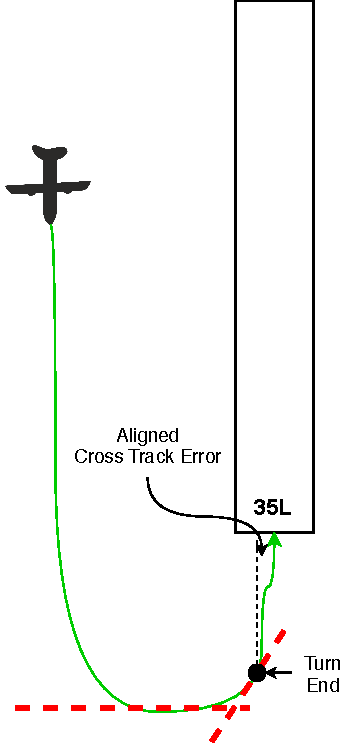
\includegraphics[width=0.29\textwidth]{img/aligned}
                }\hfill%
                \subfloat[Undershoot.  In this case, it is a small severity (Level 1) and color-coded as orange.\label{fig:undershoot_example}]{
                	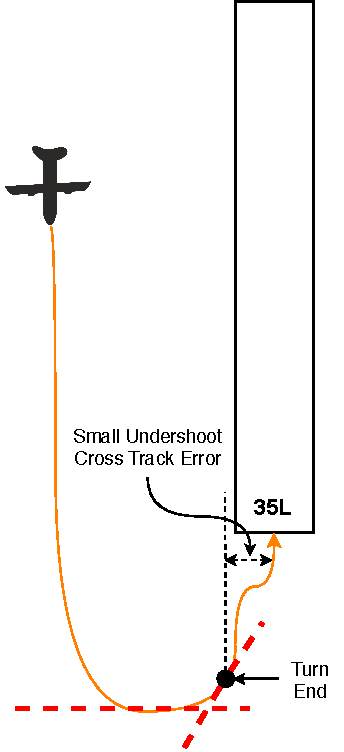
\includegraphics[width=0.29\textwidth]{img/undershoot}
                }\hfill%
                \subfloat[Overshoot.  In this case, it is a large severity (Level 2) and color-coded as red.\label{fig:overshoot_example}]{
                	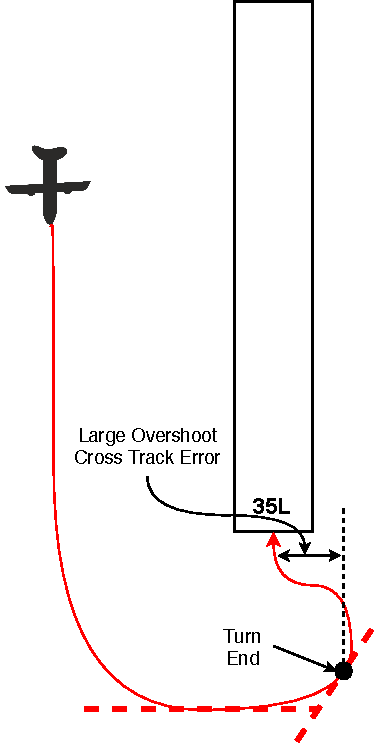
\includegraphics[width=0.29\textwidth]{img/overshoot}
                }%
                \caption{Examples showing various final turn qualities.}
                \label{fig:final_turn_examples}
            \end{figure}
            
            
            \begin{table}
            	\centering
                \caption{\small{Final turn matrix of the combinations of roll direction and cross track error.}} \label{tab:final_turn_matrix}
                \vspace{3pt}
                \begin{tabular}{|>{\bfseries}c | c c|}
                	\hline
                    \bfseries \diagbox{Direction}{Cross Track} & \bfseries $\mathbf{< 0}$\,ft & \bfseries $\mathbf{> 0}$\,ft \\
                    \hline
                    Left  & Undershoot & Overshoot \\ \hline
                    Right & Overshoot  & Undershoot \\ \hline
                \end{tabular}
            \end{table}
            
            
            %%%%% Analyze Final Turn Pseudo-code
            \begin{algorithm}
                \begin{algorithmic}[1]\raggedright
                \Function{AnalyzeFinalTurn}{startTime, endTime, runway}
                    \State $ \var{turnDataSlice} \gets $ get slice of data between \var{startTime} and \var{endTime}
                    \State $ \var{airplaneHdg} \gets \var{turnDataSlice[endTime].hdg} $
                    \State $ \var{airplanePoint} \gets \var{turnDataSlice[endTime].geoPoint} $
                    \State $ \var{crossTrackError} \gets \var{calculateCrossTrack(} \break \var{airplanePoint, airplaneHdg, runway)} $
                    
                    \State $ \var{leftDirection} \gets \abs{\var{min(turnDataSlice[`roll'])}} $
                    \State $ \var{rightDirection} \gets \abs{\var{max(turnDataSlice[`roll'])}} $
                    \If{$\var{leftDirection} > \var{rightDirection}$}
                    	\State $ \var{rollDirection} \gets $ `left'
                    \Else
                    	\State $ \var{rollDirection} \gets $ `right'
                    \EndIf
                    
                    \If{$\abs{\var{crossTrackError}} > 100$\,ft}   \Comment Level 2
                    	\State $ \var{severity} \gets $ 2
                    \ElsIf{$\abs{\var{crossTrackError}} > 25$\,ft} \Comment Level 1
                    	\State $ \var{severity} \gets $ 1
                    \Else
                    	\State $ \var{severity} \gets $ 0
                    \EndIf
                    
                    \If{\var{rollDirection} == `left'}
                        \If{$\var{crossTrackError} < 0$}
                        	\State $ \var{turnError} \gets $ `undershoot'
                        \Else
                        	\State $ \var{turnError} \gets $ `overshoot'
                        \EndIf
                    \Else
                        \If{$\var{crossTrackError} > 0$}
                        	\State $ \var{turnError} \gets $ `undershoot'
                        \Else
                        	\State $ \var{turnError} \gets $ `overshoot'
                        \EndIf
                    \EndIf
                    
                    \State $ \var{approaches[apprID]} \gets $ store severity and error
                    
                    \State \Return \var{(severity, turnError)}
                \EndFunction
                \end{algorithmic}
                \caption{Pseudo-code for function which analyzes the quality of a final turn phase.}
                \label{alg:analyze_final_turn}
            \end{algorithm}
        
        
        %----------
        % SELF-DEFINED GLIDE PATH
        %----------
        \paragraph{Self-Defined Glide Path}
        
        	A majority of runways in the U.S. publish an ideal glide slope that all pilot's should adhere to.  However, not all runways have a published glide slope.  Therefore, a method for analyzing the aircraft's actual glide path angle (GPA) during the final approach is needed in order for the pilot to be able to see what their average GPA was and how well they adhered to it.  This is why we termed this method a ``self-defined glide path angle''.  \Cref{fig:self_defined_example} shows an example of what the self-defined glide path analysis is performing.
            
            Major deviations from the ideal glide slope can be very costly.  For example, if the pilot is approaching at a steep angle, a hard landing or a landing short of the runway can occur.  On the other hand, if the pilot is approaching at a shallow angle, a runway overrun can occur.
            
            First, the slice of data for the corresponding approach phase found during the detection stage is obtained (\Cref{alg:analyze_glide_path} Line 2).  Next, a linear regression using the least squares approach is calculated (\Cref{alg:analyze_glide_path} Line 3) using the aircraft's height AGL (dependent variable) over all the time values (independent variable).  From that calculation we obtain the y-intercept, slope, and r-value (correlation coefficient) of the linear regression model (\Cref{alg:analyze_glide_path} Lines 4, 5, 15).  Then, all the necessary values for computing the pilot's defined GPA are calculated (\Cref{alg:analyze_glide_path} Lines 6-13).  Once all the supporting values are found, then the actual GPA is calculated using the $\arctan$ of the predicted vertical distance dropped over the traveled horizontal distance (\Cref{alg:analyze_glide_path} Line 14).  Furthermore, the square of the r-value is calculated (\Cref{alg:analyze_glide_path} Line 16), which explains how well the pilot's glide path ``fit'' the ideal glide path.  Lastly, the calculated values and metadata are stored in the database.
            
            
            \begin{figure}[t]
            	\centering
                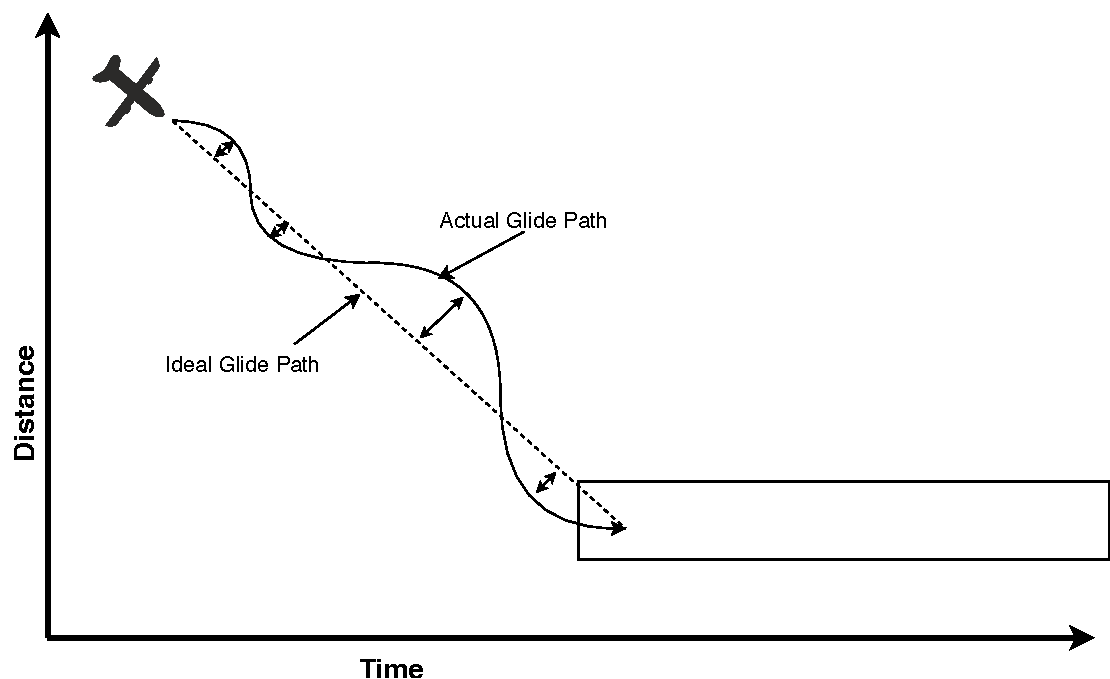
\includegraphics[width=\linewidth]{img/self_defined_example}
                \caption{Example showing the self-defined glide path angle analysis.  This shows a side view of the pilot oscillating about the glide slope during the approach phase.  The calculation uses a linear regression of the aircraft's vertical distance over time fitted using the least squares approach.  The solid line is the aircraft's actual glide path while the dotted line is the ideal glide path.}
                \label{fig:self_defined_example}
            \end{figure}
            
            
            %%%%% Analyze Self-Defined Glide Path Pseudo-code
            \begin{algorithm}[t]
                \begin{algorithmic}[1]\raggedright
                \Function{AnalyzeGlidePath}{startTime, endTime, runway}
                    \State $ \var{approachDataSlice} \gets $ get slice of data between the approach \var{startTime} and \var{endTime}
                    
                    \State $ \var{regressionResult} \gets \var{linearRegression(} \break \var{approachDataSlice[`time'], approachDataSlice[`agl'])} $
                    \State $ \var{yIntercept} \gets \var{regressionResult.intercept} $
                    \State $ \var{slope} \gets \var{regressionResult.slope} $
                    
                    \State $ \var{maxDistance} \gets \var{max(approachDataSlice[`distance'])} $
                    \State $ \var{minDistance} \gets \var{min(approachDataSlice[`distance'])} $
                    \State $ \var{horizontalDistance} \gets \var{maxDistance} - \var{minDistance} $
                    
                    \State $ \var{maxTime} \gets \var{max(approachDataSlice[`time'])} $
                    \State $ \var{minTime} \gets \var{min(approachDataSlice[`time'])} $
                    
                    \State $ \var{predictedMaxAGL} \gets \var{slope} * \var{maxTime} + \var{yIntercept} $
                    \State $ \var{predictedMinAGL} \gets \var{slope} * \var{minTime} + \var{yIntercept} $
                    
                    \State $ \var{predictedVerticalDistance} \gets \var{predictedMaxAGL} - \var{predictedMinAGL} $
                    
                    \State $ \var{actualGlidePathAngle} \gets \var{degrees(} \break \var{atan(predictedVerticalDistance / horizontalDistance))} $
                    
                    \State $ \var{pearsonsR} \gets \var{regressionResult.rvalue} $
                    \State $ \var{rSquared} \gets \var{pearsonsR} * \var{pearsonsR} $
                    
                    \State $ \var{approaches[apprID]} \gets $ store self-defined glide path metadata
                    \State \Return \var{(actualGlidePathAngle, rSquared)}
                \EndFunction
                \end{algorithmic}
                \caption{Pseudo-code for function which analyzes the quality of the aircraft's glide path angle during the approach phase.}
                \label{alg:analyze_glide_path}
            \end{algorithm}
    

%----------------------------------------
% GRADING METRICS
%----------------------------------------
\subsection{Grading Metrics}
    
    When creating the risk level metrics to be used for grading the approach analysis data, we wanted to ensure they were backed by statistics obtained from the results from the sample set of flights.  Towards that goal, the risk level metrics have been created from the data found during the approach quality analysis.  For each parameter of concern, the recorded values across all approach phases in the sample set were used to create a normalized histogram showing the probability density of each value range.  From these histograms, the mean and standard deviation were calculated in order to create a best-fit line to overlay the histogram.  The charts were then analyzed by an aviation statistics expert at the University of North Dakota who gave his opinion on reasonable values to use for Risk Level 1 and 2 value ranges based on each mean, standard deviation, and best-fit line.  Even though those elements were created from the analysis statistics, the aviation expert wanted to also ensure the safe value ranges (Risk Level 0) did not conflict with the values published in UND's standardization manual~\cite{und_flight_manual} and the Cessna C172S Pilot's Operating Handbook (POH)~\cite{und_poh}.
    
    After the risk level metrics have been established, the approach quality analysis results will be re-processed and graded according to the metrics.  The resulting grade is then stored along with the other generated approach analysis data within the database.  The specific details of the grading results from using the risk level metrics will be discussed further in \Cref{ch:results}.
    
    
%----------------------------------------
% WEB INTERFACES
%----------------------------------------
\subsection{Web Interfaces}

	This Section details the newly developed web pages for the NGAFID, which dynamically display results based on the user's chosen filters.  At the time of this writing, there have been new tools developed for each of the approach, final turn, and self-defined glide path analyses.  Each tool will be discussed further in the subsequent Subsections.
    
    
    %----------
    % APPROACH
    %----------
    \subsubsection{Approach}
    
    	A new web page was implemented in the NGAFID for the purpose of dynamically displaying the approach analysis results produced by the \toolname\ to users (\Cref{fig:approach_tool_screenshot}).  The results are given in four tabs, one for each parameter, as histograms over a specified date range.  A user is able to dynamically add additional date ranges, which will create an additional series in the chart for comparison.  This feature can be used to detect changes in trends over time.  A user is also, optionally, able to filter the results to an airport and further filter to a single runway.  This will allow users to identify trends that are potentially occurring at a specific runway but not at any other runways.
    
    	\begin{figure}
    		\centering
            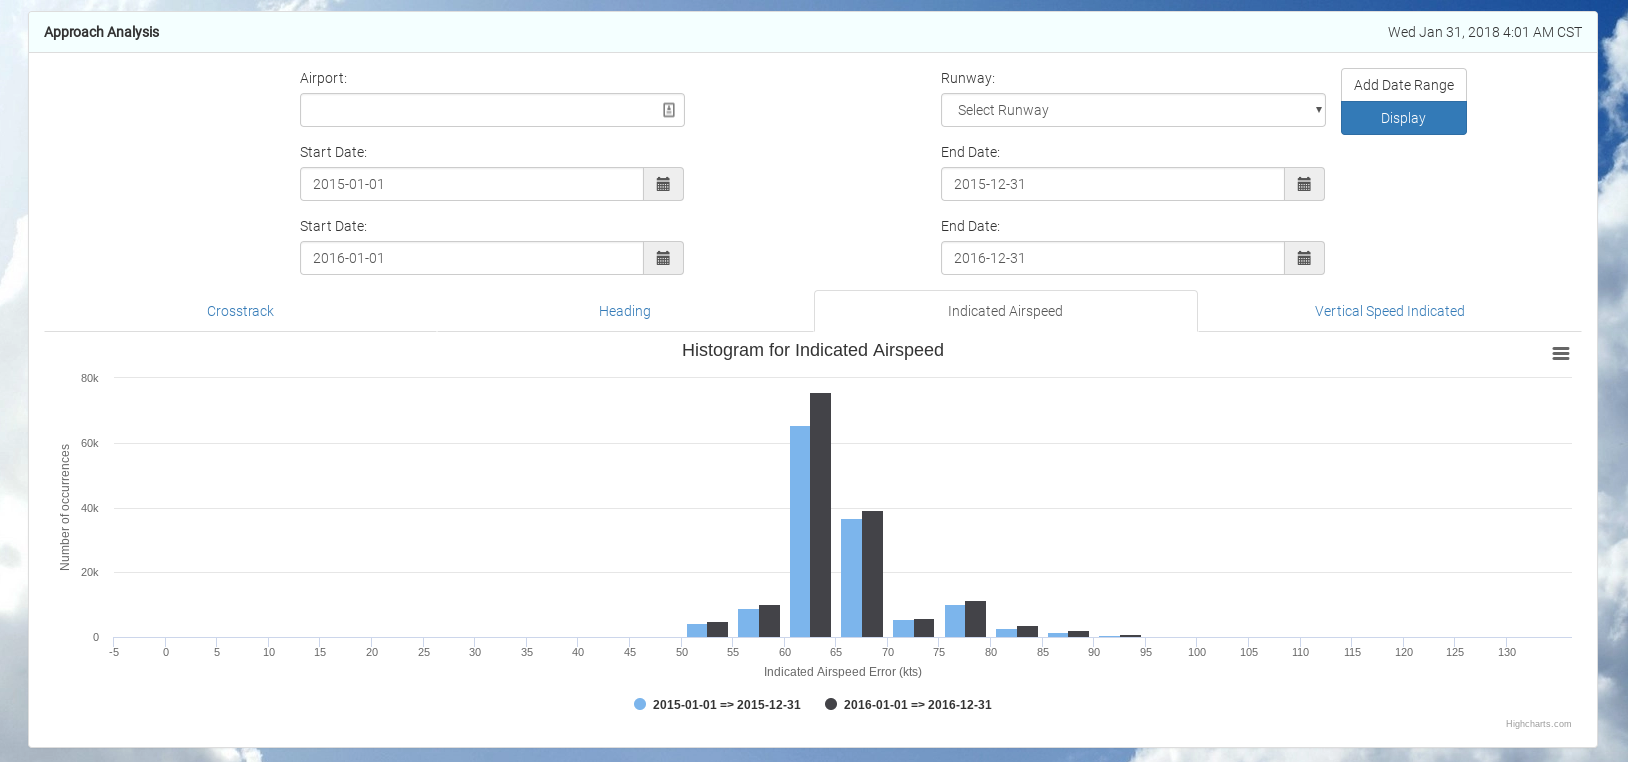
\includegraphics[width=\linewidth]{img/approach_tool_screenshot}
            \caption{A screenshot of the Approach analysis tool on the NGAFID.  It is showing the histogram for indicated airspeed error with two date range filters: 2015-01-01 to 2015-12-31 and 2016-01-01 to 2016-12-31.  The frequency of exceedances can be seen with all values that fall outside of the 55-75 knots range.}
            \label{fig:approach_tool_screenshot}
    	\end{figure}
    
    
    %----------
    % FINAL TURN
    %----------
    \subsubsection{Final Turn}
    
    	The tool developed for analyzing final turn phases in the NGAFID was implemented with two modes:  \textit{(i)} ``Single Flight'' and \textit{(ii)} ``Aggregate''.
    
    	For the ``Single Flight'' mode, the user can input an ID for a specific flight they'd like to analyze (\Cref{fig:single_ttf_screenshot}).  Once the user clicks the ``Display Single Flight'' button, the interactive map then dynamically transitions to the first approach for that flight.  The map will only display one approach at a time; although, there are tabs across the top for each approach which the user can choose.  Once a different tab is chosen, the map automatically transitions the view to that corresponding approach.  The flight path shows different color codings for the separate final turn, approach, and landing phases as well as different colors for the final turn specifically depending on the severity of the turn error.  A Level 1 turn error will be colored yellow, while a Level 2 turn error will be colored red.  If the turn error is less than the Level 1 criteria, it is colored green.  The user is also able to download a PNG screenshot of the map by clicking the ``Download PNG'' button.
        
        For the ``Aggregate'' mode; the user can choose a specific airport, runway, and month and year combination; which will then display all the approaches that occurred at the chosen runway during the chosen time-frame (\Cref{fig:agg_ttf_screenshot}).  This mode allows a user to see trends in final turn phases during a given time span.  This mode displays the same color code scheme as the ``Single Flight'' mode.
    
    	\begin{figure}
    		\centering
            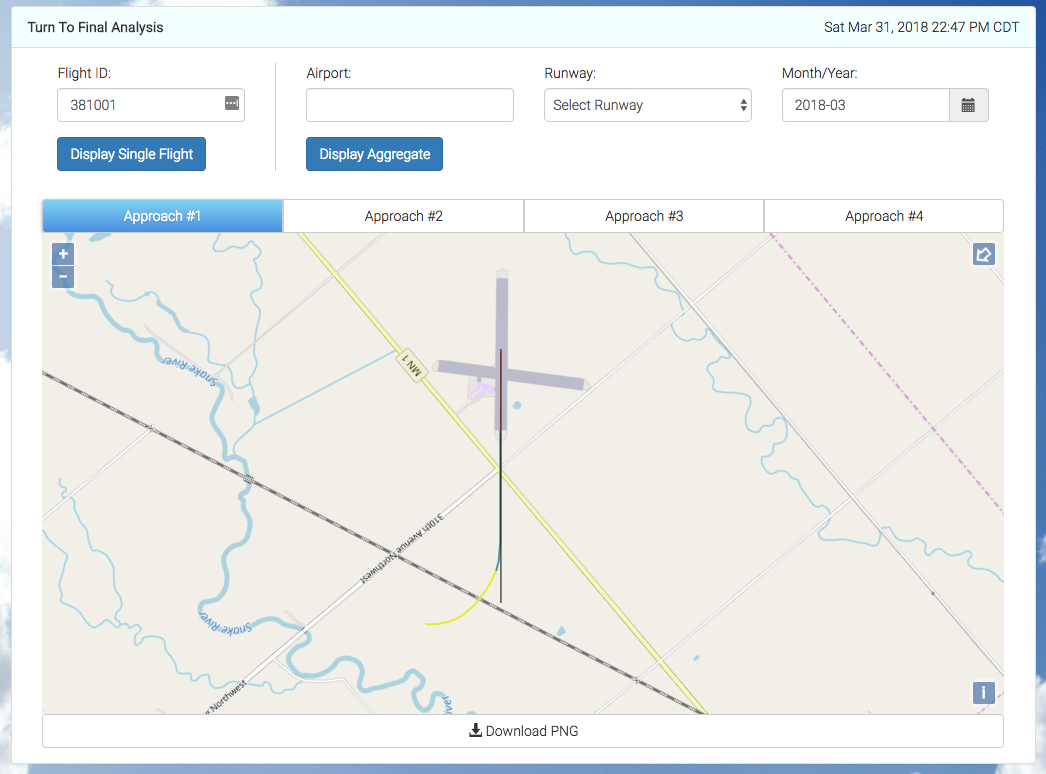
\includegraphics[width=\linewidth]{img/single_ttf_screenshot}
            \caption{A screenshot of the Final Turn analysis tool on the NGAFID in ``Single Flight'' mode.  It is currently showing approach \#1 for Flight ID \#381001.  Approach \#1 shown here had a Level 1 (yellow color code) undershoot.}
            \label{fig:single_ttf_screenshot}
    	\end{figure}
        
        \begin{figure}
    		\centering
            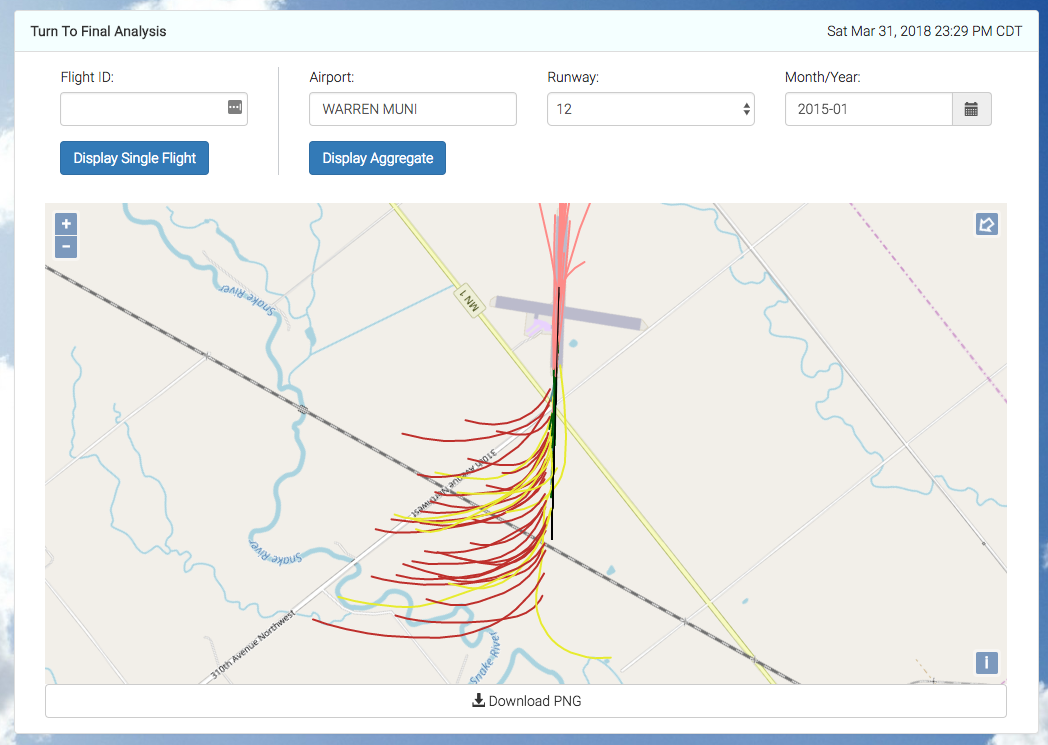
\includegraphics[width=\linewidth]{img/agg_ttf_screenshot}
            \caption{A screenshot of the Final Turn analysis tool on the NGAFID in ``Aggregate'' mode.  It is currently showing all approaches at the Warren Municipal Airport (KD37) for Runway 12 during the month of January 2015.  The many red and yellow lines coming in from the left side mean that a majority of the turns were Level 1 \& 2 undershoots.}
            \label{fig:agg_ttf_screenshot}
    	\end{figure}
    
    %----------
    % SELF-DEFINED
    %----------
    \subsubsection{Self-Defined Glide Path}
    
    	The tool implemented in the NGAFID for displaying the results of the self-defined glide path analysis currently only supports an aggregate mode (\Cref{fig:self_defined_screenshot}).  It works similarly to the final turn tool as the user chooses an airport, runway, and month and year combination.  This will then display a sideways histogram of all the approaches at the given runway during the given time-frame.  The y-axis shows glide path angles from $0^\circ$ to $10^\circ$ in $0.5^\circ$ increments, and the x-axis shows the number of occurrences that fell within each angle bin.  Lastly, the user can download an image of the displayed chart by clicking the ``hamburger'' menu button.
    
    	\begin{figure}
    		\centering
            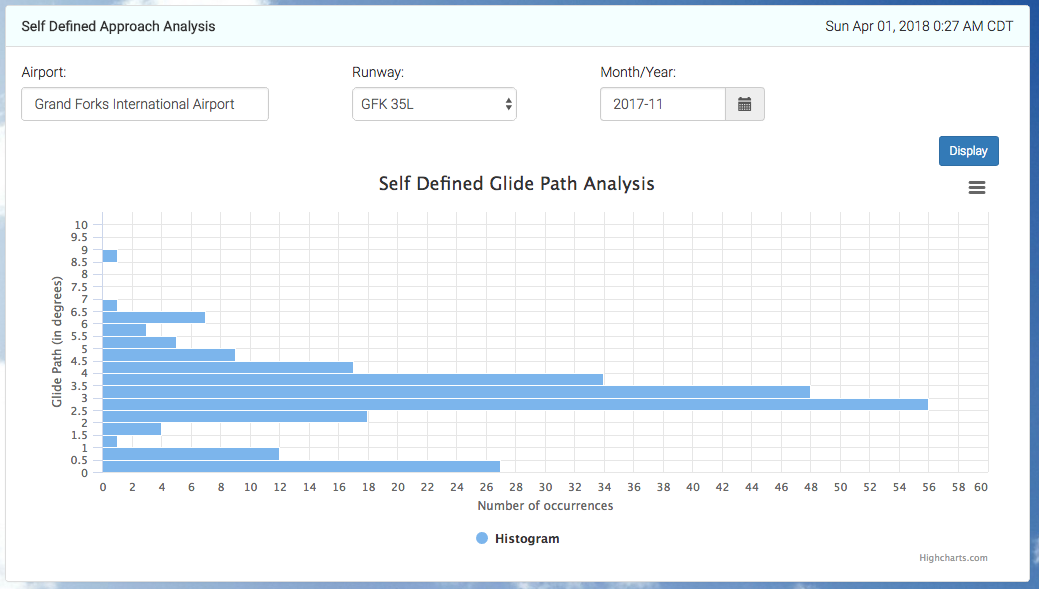
\includegraphics[width=\linewidth]{img/self_defined_screenshot}
            \caption{A screenshot of the Self-Defined Approach analysis tool on the NGAFID.  It is currently showing all approaches at the Grand Forks International Airport (KGFK) for Runway 35L during the month of November 2017.  It displays a sideways histogram with glide path angles on the y-axis and the number of occurrences for each angle on the x-axis.}
            \label{fig:self_defined_screenshot}
    	\end{figure}



% !TEX root =  ../main.tex

\section{Implementation} \label{sec:implementation}

%----------------------------------------
% PROGRAMMING LANGUAGES & LIBRARIES
%----------------------------------------
\subsection{Programming Languages and Libraries}

	The Python programming language was used for implementing the flight analysis due to its ease of use, its reputable scientific and graphing libraries, and the ability to quickly produce a viable application.  The libraries utilized are MySQLdb\footnote{v1.3.12: http://mysql-python.sourceforge.net/MySQLdb.html} for interacting with the MySQL database; matplotlib\footnote{v2.2.2: https://matplotlib.org/} for graphing flight parameters in the early stages of the application; NumPy\footnote{v1.14.0: http://www.numpy.org/}, Scipy\footnote{v1.0.0: https://docs.scipy.org/doc/scipy/reference/index.html}, and Pandas\footnote{v0.22.0: https://pandas.pydata.org/} for their scientific and vectorized functions; and the geodesy scripts created by Chris Veness\footnote{http://www.movable-type.co.uk/scripts/latlong.html}.  All source code is available at \url{https://github.com/KeltonKarboviak/NGAFID}.
    
    For the back-end of the web interface, Laravel\footnote{v5.0: https://laravel.com/} was used as the PHP framework.  For the front-end, the following technologies were used:  jQuery\footnote{v2.2.4: https://jquery.com/} \& jQuery UI\footnote{v1.11.2: https://jqueryui.com/}, Bootstrap\footnote{v3: https://getbootstrap.com/docs/3.3/} for CSS styling, OpenLayers\footnote{v4.6.4: http://openlayers.org/} for creating an interactive map, OpenStreetMap\footnote{https://www.openstreetmap.org} for the images used by OpenLayers, and Turf.js\footnote{v5.1.5: http://turfjs.org/} for its geodesy functions.  All source code for the web interface is available at \url{https://github.com/travisdesell/ngafid}.


%----------------------------------------
% HARDWARE SPECS
%----------------------------------------
\subsection{Hardware Specs}

	All experiments were performed on a 2013 Mac Pro running macOS 10.11.6 with a 3.5 GHz 6 hyper-threaded core Intel Xeon E5 processor (for a total of 12 logical processing cores). The machine also has 32 GBs of 1866 MHz DDR3 ECC RAM.


%----------------------------------------
% PARALLELIZATION
%----------------------------------------
\subsection{Parallelization} \label{sec:parallelization}

	The application was originally created to process the flight data in a linear fashion.  This proved to be fairly time consuming when running the application in batch mode with the significant number of flights contained in the NGAFID.  In order to improve the performance and efficiency of the application, Python's built-in multiprocessing module was used.  The parallel application uses the Producer-Consumer model in which the parent process acts at the Producer by enqueuing all of the unique flight identifiers onto a queue and the child subprocesses act as the Consumers by dequeuing a flight identifier then processing it.  The multiprocessing module was chosen over the built-in threading module due to the issue with Python's Global Interpreter Lock (GIL) effectively restricting bytecode execution to a single core~\cite{beazley2010understanding}.  This makes the threading module unusable for long-running CPU-bound tasks, which this application heavily relies on.
	
% !TEX root = ../main.tex

\section{Results} \label{sec:results}

%----------------------------------------
% EXPERIMENTS
%----------------------------------------
\subsection{Experiments}

	The experiments were run using Cessna 172S flight data produced by students at the University of North Dakota during the month of September 2015.  Student flight data is ideal for unstable analysis testing as it contains very noisy data, which provides a diverse array of flying patterns.  A random sample of 100 flights was chosen for the experiments.
        
    First, the application was run against the 100 flights to obtain the automated analysis results.  The same 100 flights were then manually analyzed in order to get human results for the phase identification, which could be compared to the automated results then determine the accuracy of the application.  The test of the 100 flights was also run ten times each with the single-process version and the multi-process version as previously described.  This was done in order to compare and contrast the performance of the separate versions.


%----------------------------------------
% ACCURACY OF PHASE IDENTIFICATION
%----------------------------------------
\subsection{Accuracy of Phase Identification}

	The manual validation was performed using a combination of tools available on the NGAFID website:  the Cesium flight reanimation tool and the Keyhole Markup Language (KML) generator to visualize the flight path in \textit{Google Earth}~\cite{nolan2014keyhole} (see \Cref{fig:kml_example}).
    
    \begin{figure}
    	\centering
        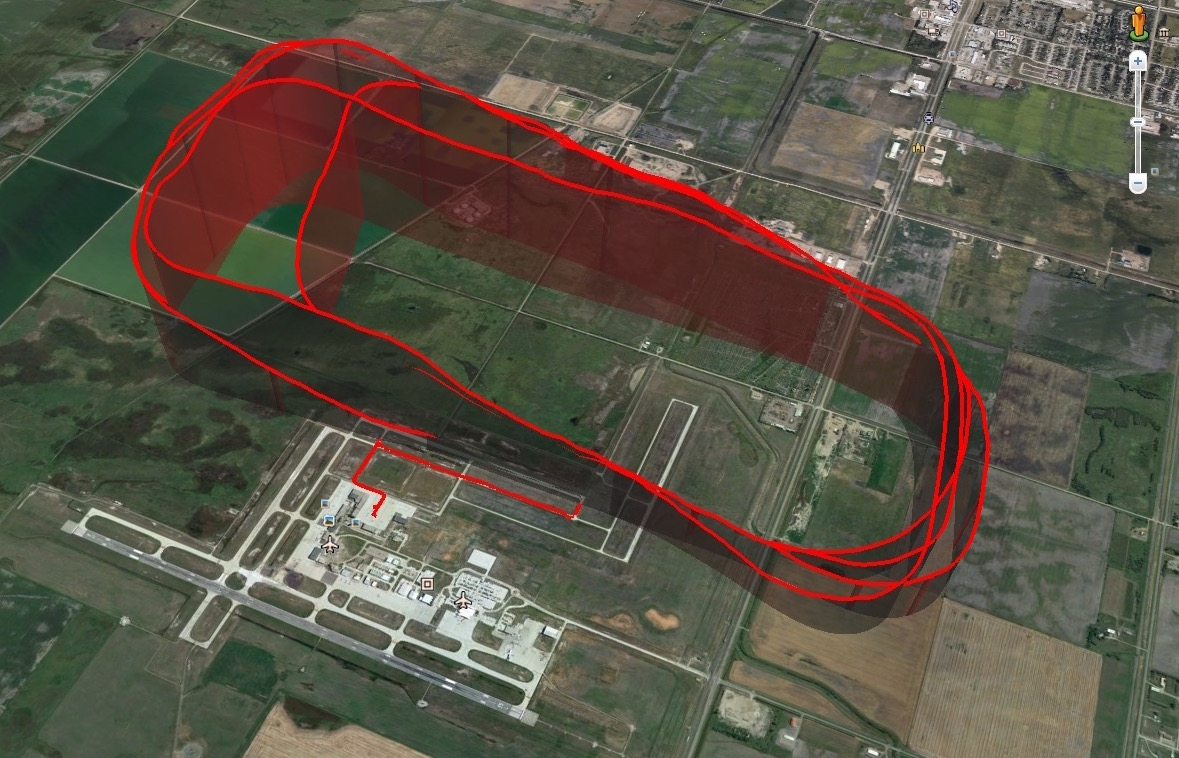
\includegraphics[width=\linewidth]{kml_example}
        \caption{Example of using a KML file to visualize a flight path in \textit{Google Earth}.  This flight visualization is an example of a student flight that has multiple approach phases.}
        \label{fig:kml_example}
    \end{figure}
    
    
    %----------
    % APPROACH
    %----------
    \subsubsection{Approach}
    
        The \toolname\ generated a total of 380 approaches for the 100 flights that were tested. As seen in \Cref{fig:kml_example}, student flights typically consist of multiple approaches as this is something that needs to be practiced.  Out of the total; there are 373 (98.16\%) true positives, five (1.32\%) false positives, and two (0.53\%) false negatives.  These results can also be found in \Cref{fig:validation_results}.
        
        In the context of this application, a true positive is a case where the tool correctly indicates that an approach is occurring during a specified time frame.
        
        A false positive occurs when the tool indicates that an approach is occurring but is not in reality.  Typically, a false positive occurs when the flight data has invalid values for about the first ten rows, which then throws off the beginning of the algorithms.  This happens infrequently, but could be accounted for in a future work by sanitizing the data before analysis.
        
        A false negative is the exact opposite where the tool indicates that an approach is not occurring but it is in reality.  Typically, a false negative occurs when the approached runway's geological data is not contained within the database.  These types of occurrences should stop once the airport and runway databases are expanded with more entries.
        
        The tool misclassified the approached runway 13 times (3.42\%).  A runway is misclassified when the difference between the aircraft and runway headings is greater than $20^\circ$.  This occurs during the runway detection portion of the approach analysis algorithm, and the algorithm either returns a \emph{null} runway or an incorrect runway due to the large heading difference.  Lastly, there was a total of 42 (11.05\%) approaches that were given a \textit{null} runway.  This number overlaps with some of the 13 misclassifications, while the rest are due to a lack of runway information as mentioned previously.

        In this same context, it is difficult to quantify the number of true negatives since these would be cases where the tool correctly indicates that an approach is not occurring.  The difficulty lies in how to define a single occurrence.  Should a single true negative be counted for every second the tool indicates that an approach is not occurring?  If so, then this would create a numerous amount of true negatives and would dilute the percentages of the other statistics, which are more important in this application.

        The validation results demonstrate that the \toolname\ is exceptionally accurate in its ability to appropriately detect and classify most approaches in a flight.

        \begin{figure}
            \centering
            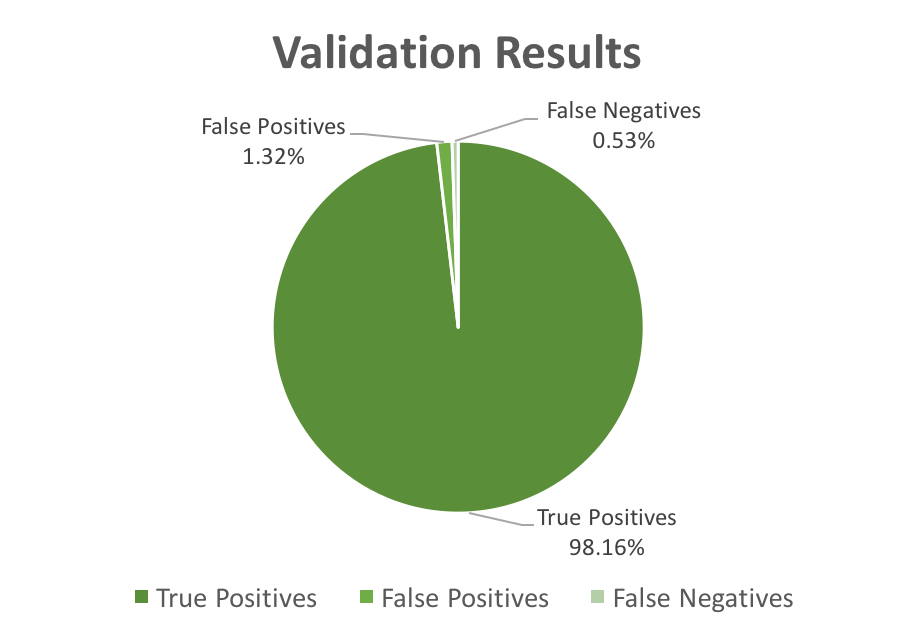
\includegraphics[width=0.85\linewidth]{validation_results}
            \caption{Pie chart showing the manual validation results including true positives, false positives, and false negatives.}
            \label{fig:validation_results}
        \end{figure}
    
    
%----------------------------------------
% QUALITY ANALYSIS RESULTS
%----------------------------------------
\subsection{Quality Analysis}


	%----------
    % APPROACH
    %----------
    \subsubsection{Approach}
    
    	The results of the application have provided many possibilities for statistical analysis since numerous statistics can be calculated from the generated approach data.  This can be seen in \Cref{subfig:stableness_results,subfig:unstable_landing_results,subfig:unstable_parameters,subfig:landing_type_results} in which a sample of the possible results were calculated from the experiments of the 100 flights used in this research.  With these various results, trends can be found in the data that has been analyzed.  For example, we can see in \Cref{subfig:stableness_results} that out of the 380 approaches in the sample data, 57.11\% (217) were stable and 42.89\% (163) were unstable.  By drilling down into that data, we can see the frequency for each of the landing types for stable and unstable approaches.  \Cref{subfig:landing_type_results} depicts this more detailed information and shows that full-stop landings occur most frequently for both stable and unstable approaches.  This result is not very surprising for stable approaches; however, it is very undesirable for unstable approaches.  If we look even further into the proportions for unstable approaches alone (\Cref{subfig:unstable_landing_results}), we see that an unstable approach resulted in a go-around only 34.97\% of the time.  This is far lower than the hopeful 100\%, but was expected to be approximately 20\% by our aviation safety experts.  As mentioned previously, this is largely due to pilot misjudgment since all the analyzed flights were piloted by aviation students; meaning they are still learning and are not yet professionals.
    
    When looking at the unstable approaches and the parameters that caused them (\Cref{subfig:unstable_parameters}), additional interesting results can be found.  We found the parameter that was exceeded the most was heading with 91 occurrences.  Heading was not predicted to be the leading cause of unstable approaches, but our safety experts believe the 10$^\circ$ threshold (as defined in \Cref{tab:approach_thresholds}) may be too strict.  Indicated airspeed was the second highest, but was predicted to be the leading cause since it was stated by our aviation safety experts to be a trend for UND's student pilots to be going too fast on final approaches.
    
    \begin{figure}
    	\centering
        \subfloat[Pie chart showing the number of stable approaches compared to the number of unstable approaches.\label{subfig:stableness_results}]{
        	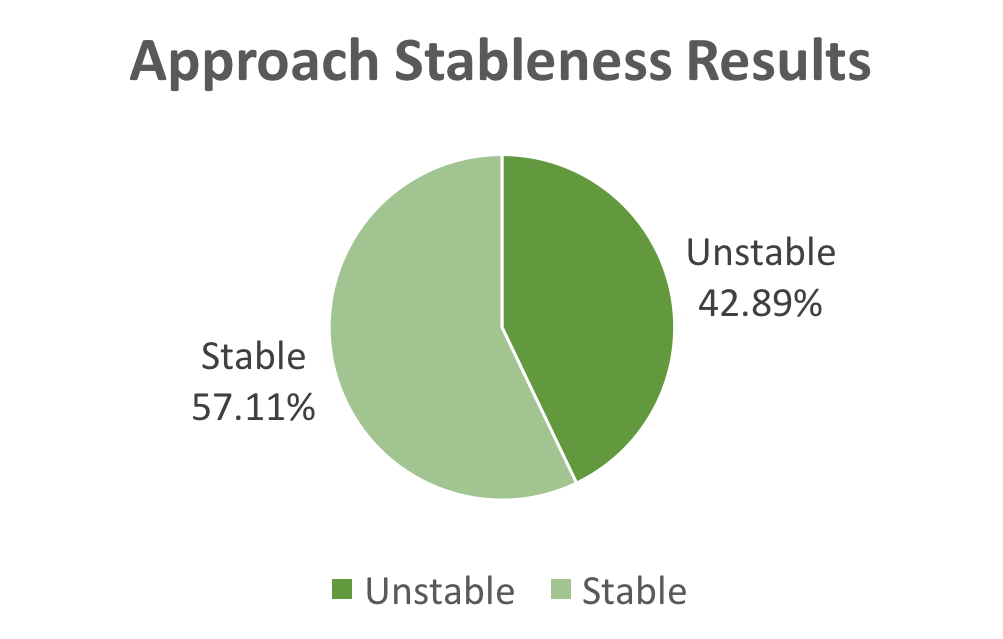
\includegraphics[width=0.45\linewidth]{stableness_results}
        }\hfill%
        \subfloat[Frequency of the occurrences of each landing type for stable and unstable approaches.\label{subfig:landing_type_results}]{
        	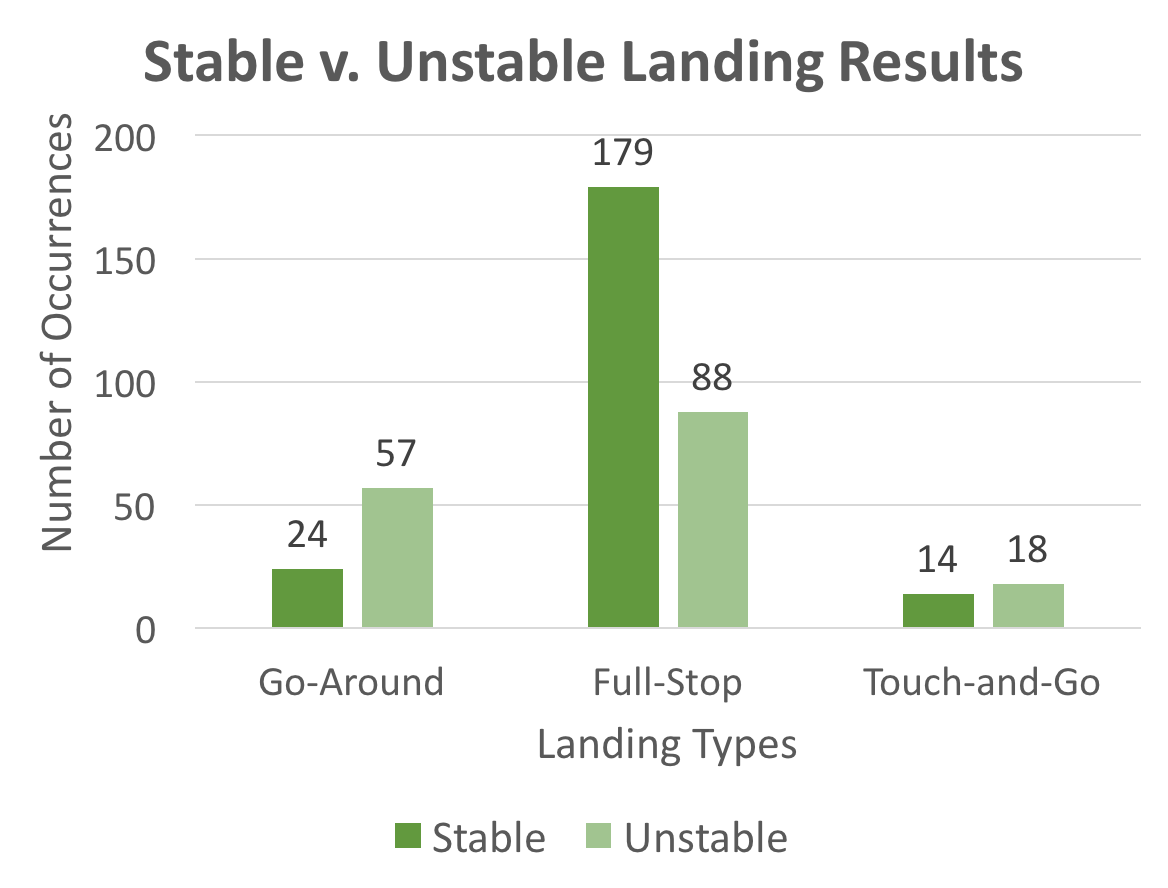
\includegraphics[width=0.45\linewidth]{landing_type_results}
        }%
        
        \subfloat[Pie chart comparing the number of occurrences for each landing type after an unstable approach.\label{subfig:unstable_landing_results}]{
        	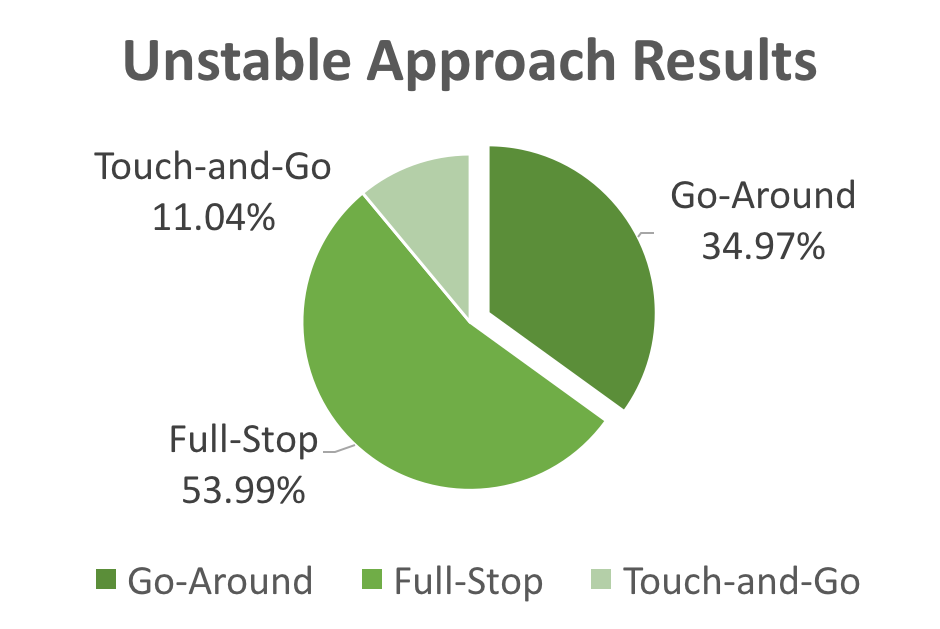
\includegraphics[width=0.45\linewidth]{img/unstable_approach_landing_results}
        }\hfill%
        \subfloat[Frequency of parameters that caused an aircraft to be unstable during an approach.  Note that a single approach can have multiple unstable parameters, which causes the sum of the occurrences to not equal the total number of unstable approaches.\label{subfig:unstable_parameters}]{
        	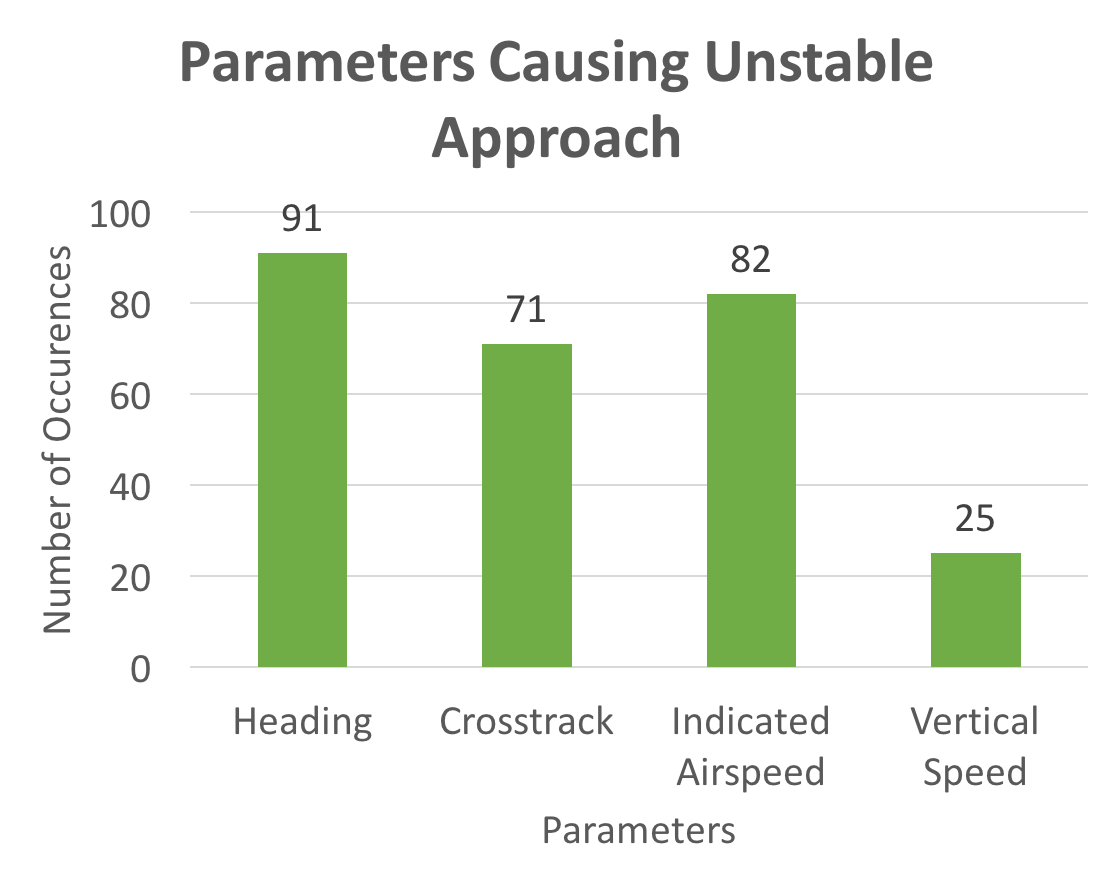
\includegraphics[width=0.45\linewidth]{unstable_parameter_results}
        }%
        \caption{Sample set of the statistics and trends that can be found from the automated analysis results.}
        \label{fig:example_statistics}
    \end{figure}
    
    
    Another interesting set of statistics that can be drawn from the analysis are parameter value frequencies.  Creating histograms of the values for each parameter during all approach phases can show the values that occur most frequently (highest density).  \Cref{subfig:approach_ias_hist,subfig:approach_vsi_hist,subfig:approach_cross_track_hist,subfig:approach_heading_hist} visualize these histograms and give the corresponding mean and standard deviation values.  These graphs are able to show how well pilots are adhering to the published stabilized approach criteria (see \Cref{tab:approach_thresholds}).  As mentioned previously, the standard deviations will be used in defining the grading metrics and will be discussed in more detail later in this Chapter.
    
    \begin{figure}
    	\centering
        \subfloat[Indicated airspeed.\label{subfig:approach_ias_hist}]{
        	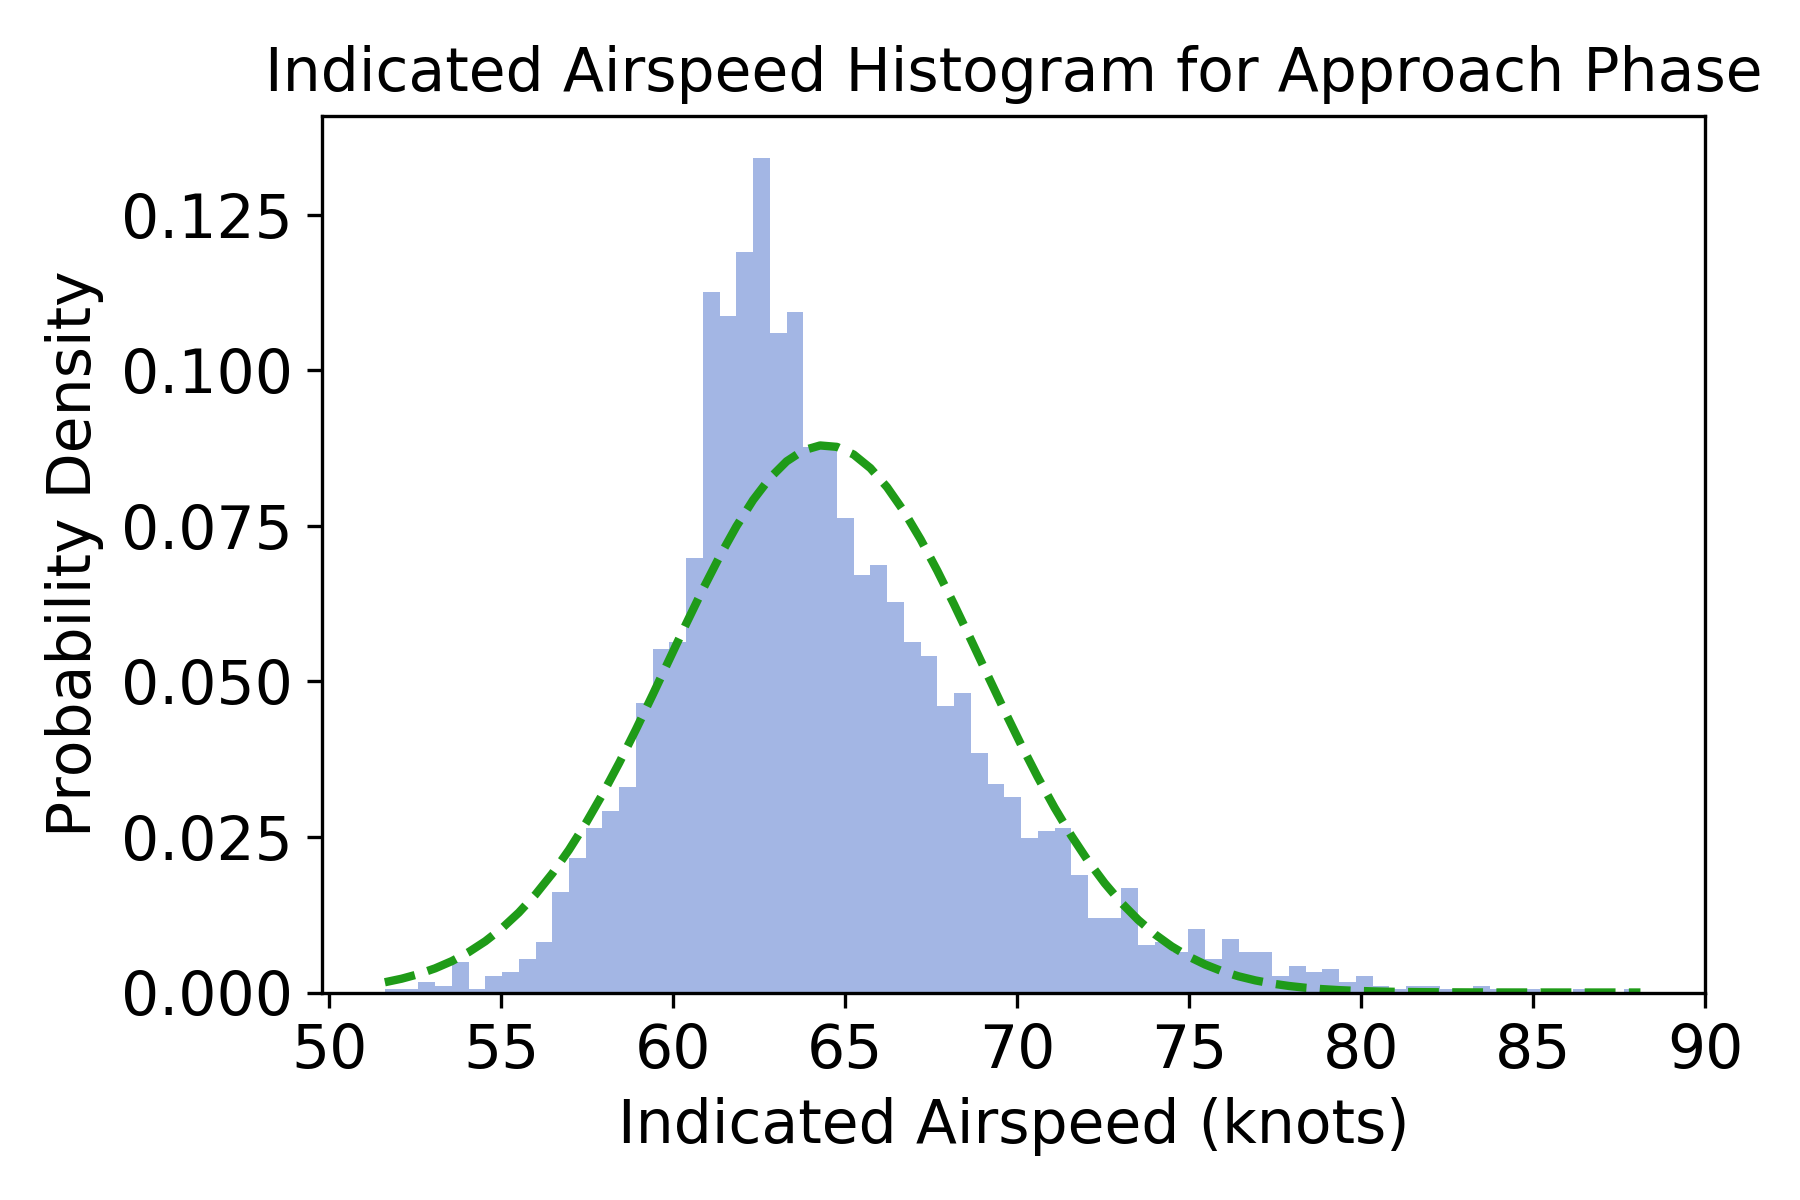
\includegraphics[width=0.45\linewidth]{orig_ias_hist}
        }\hfill%
        \subfloat[Vertical speed indicated.\label{subfig:approach_vsi_hist}]{
        	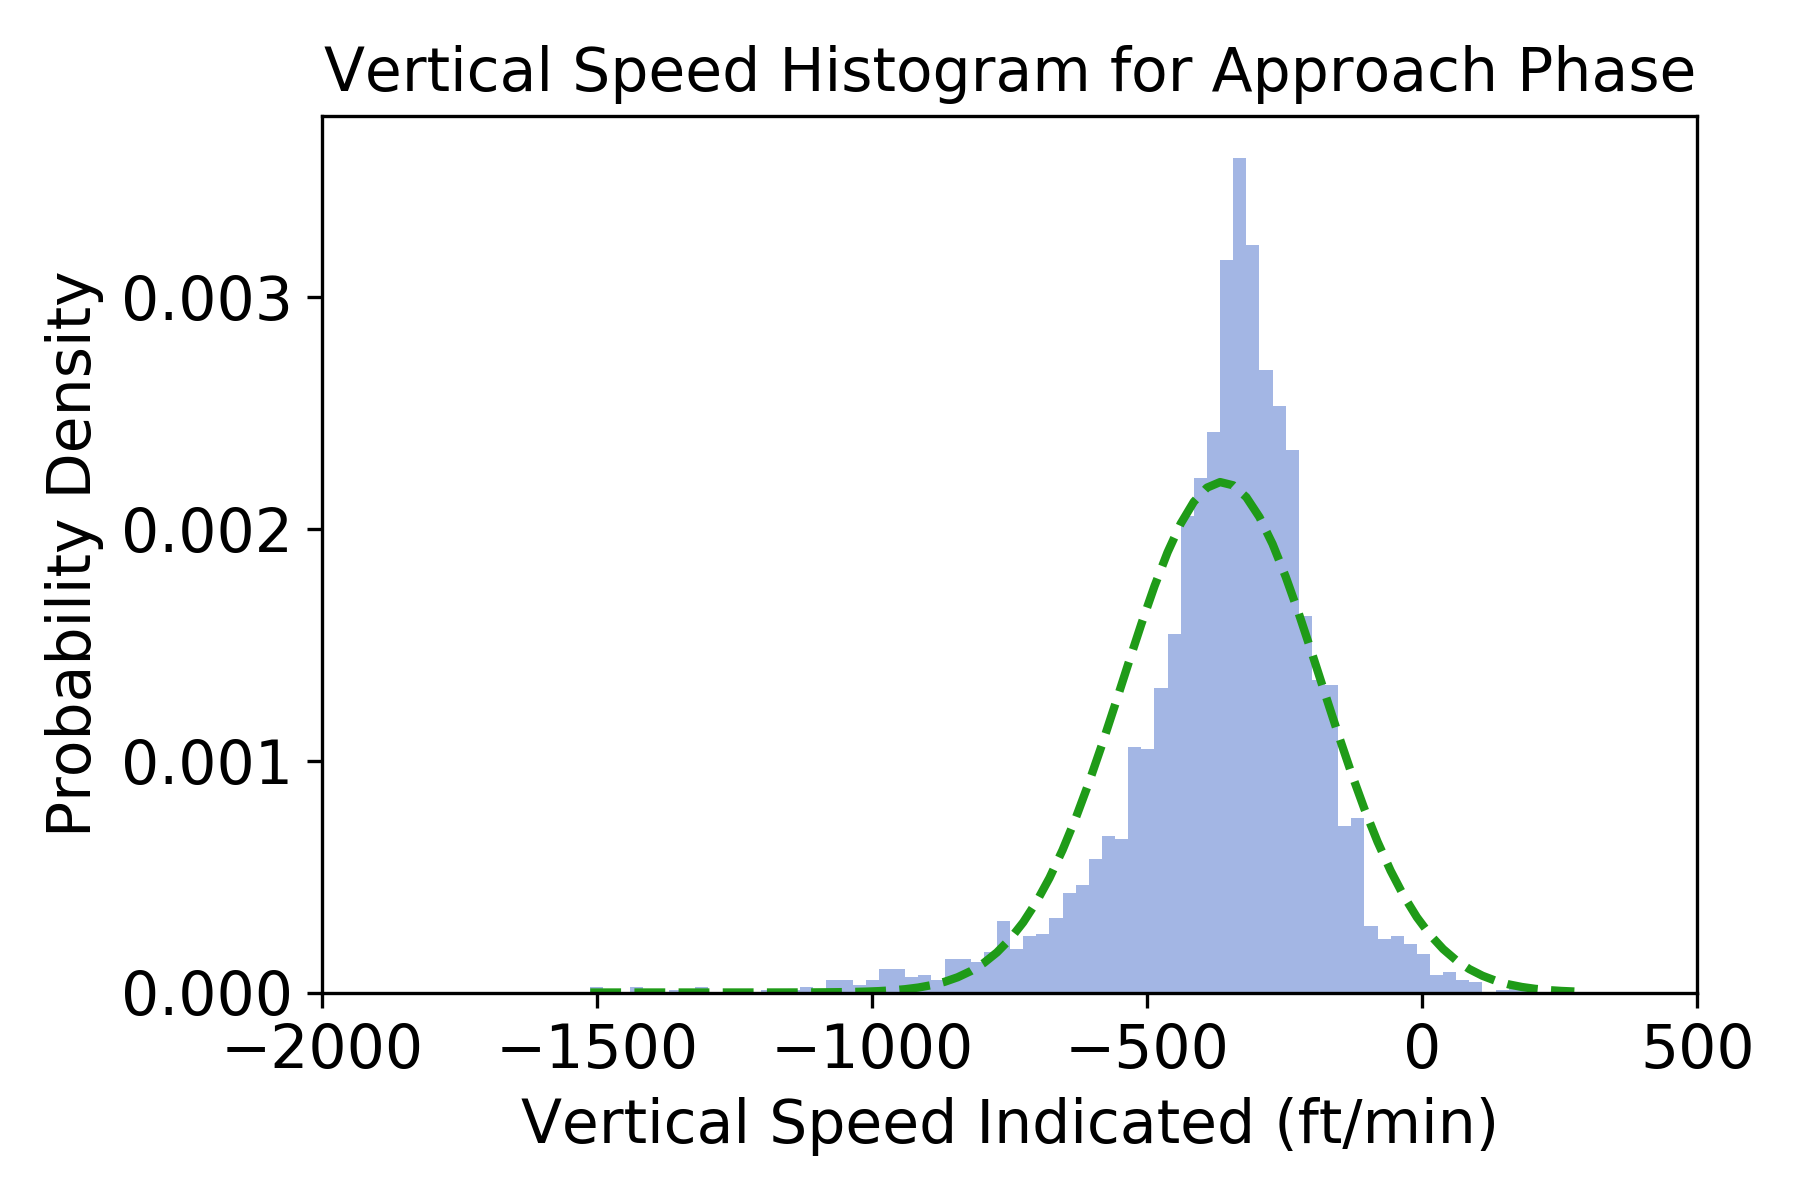
\includegraphics[width=0.45\linewidth]{orig_vsi_hist}
        }%
        
        \subfloat[Cross track error.\label{subfig:approach_cross_track_hist}]{
        	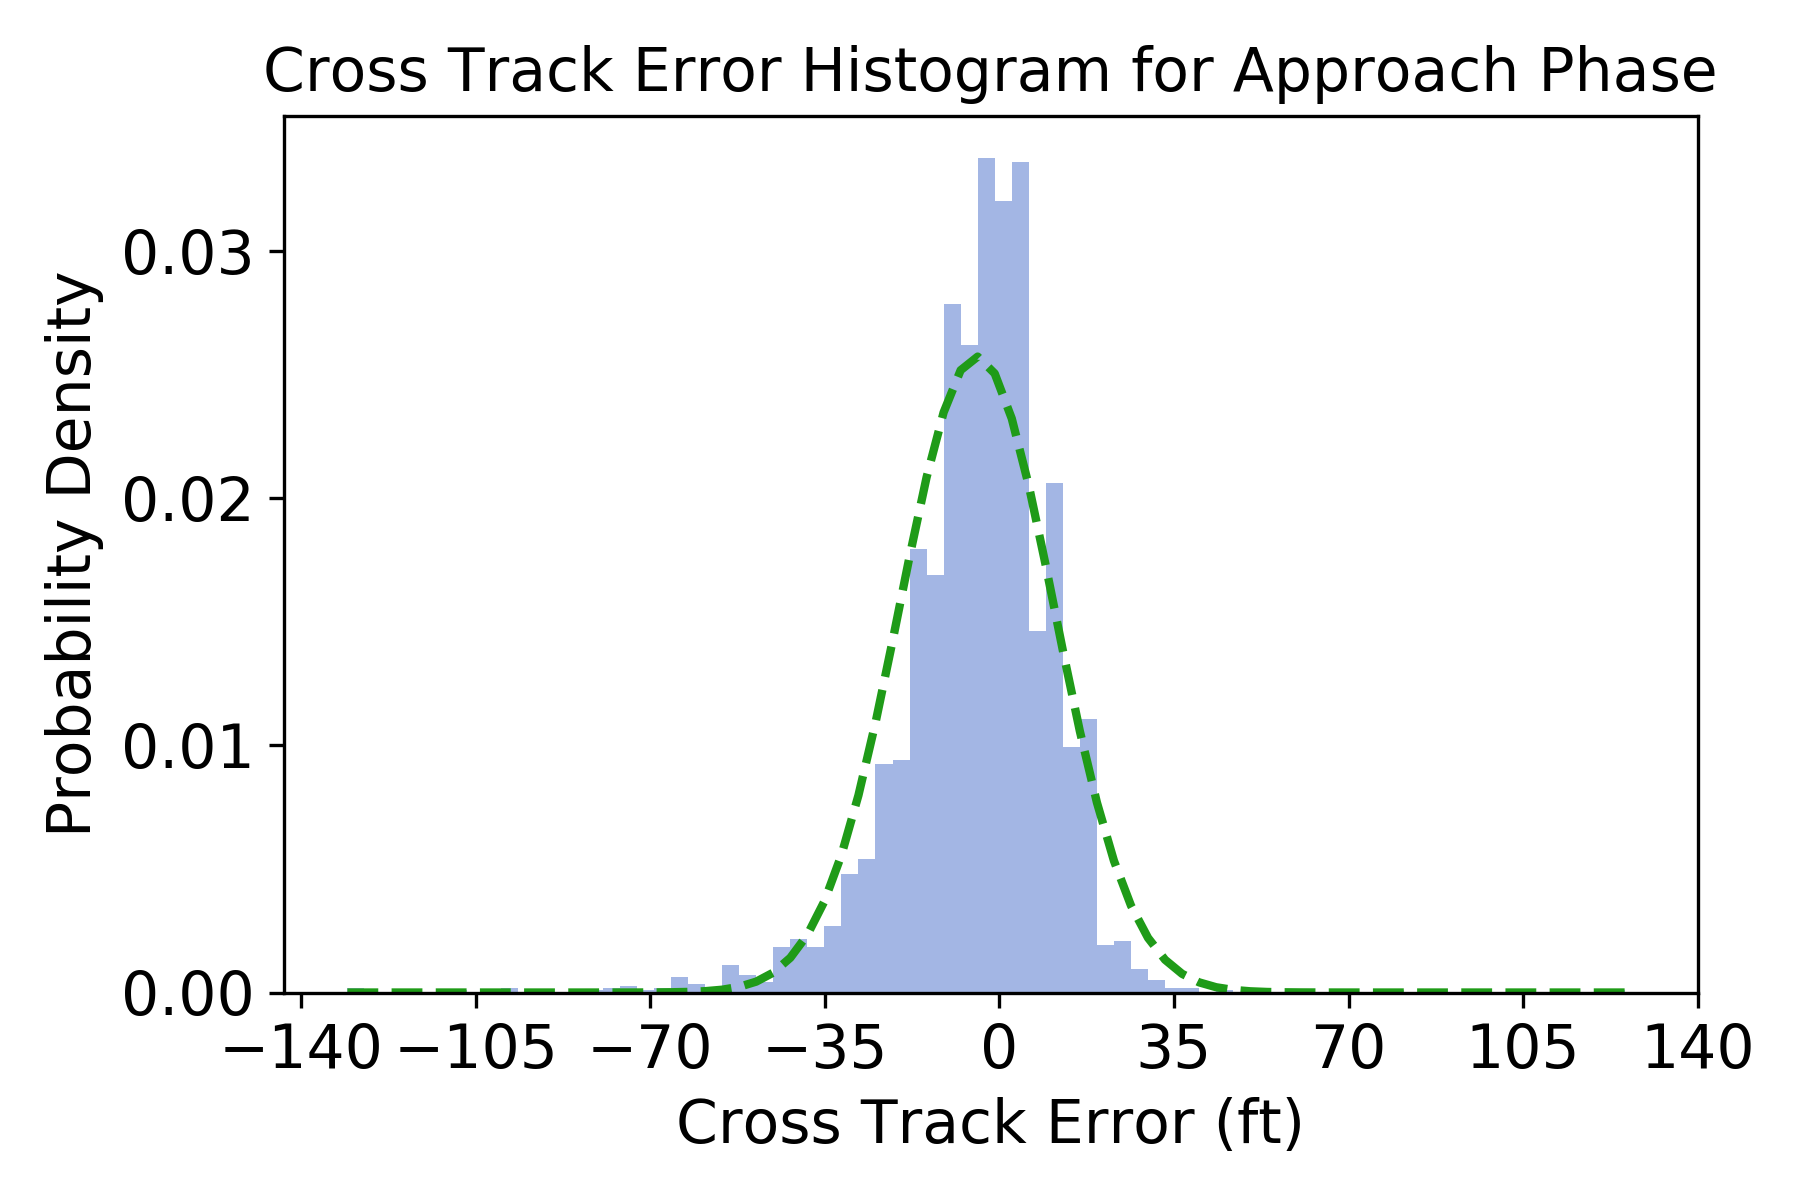
\includegraphics[width=0.45\linewidth]{orig_cross_track_hist}
        }\hfill%
        \subfloat[Heading error.\label{subfig:approach_heading_hist}]{
        	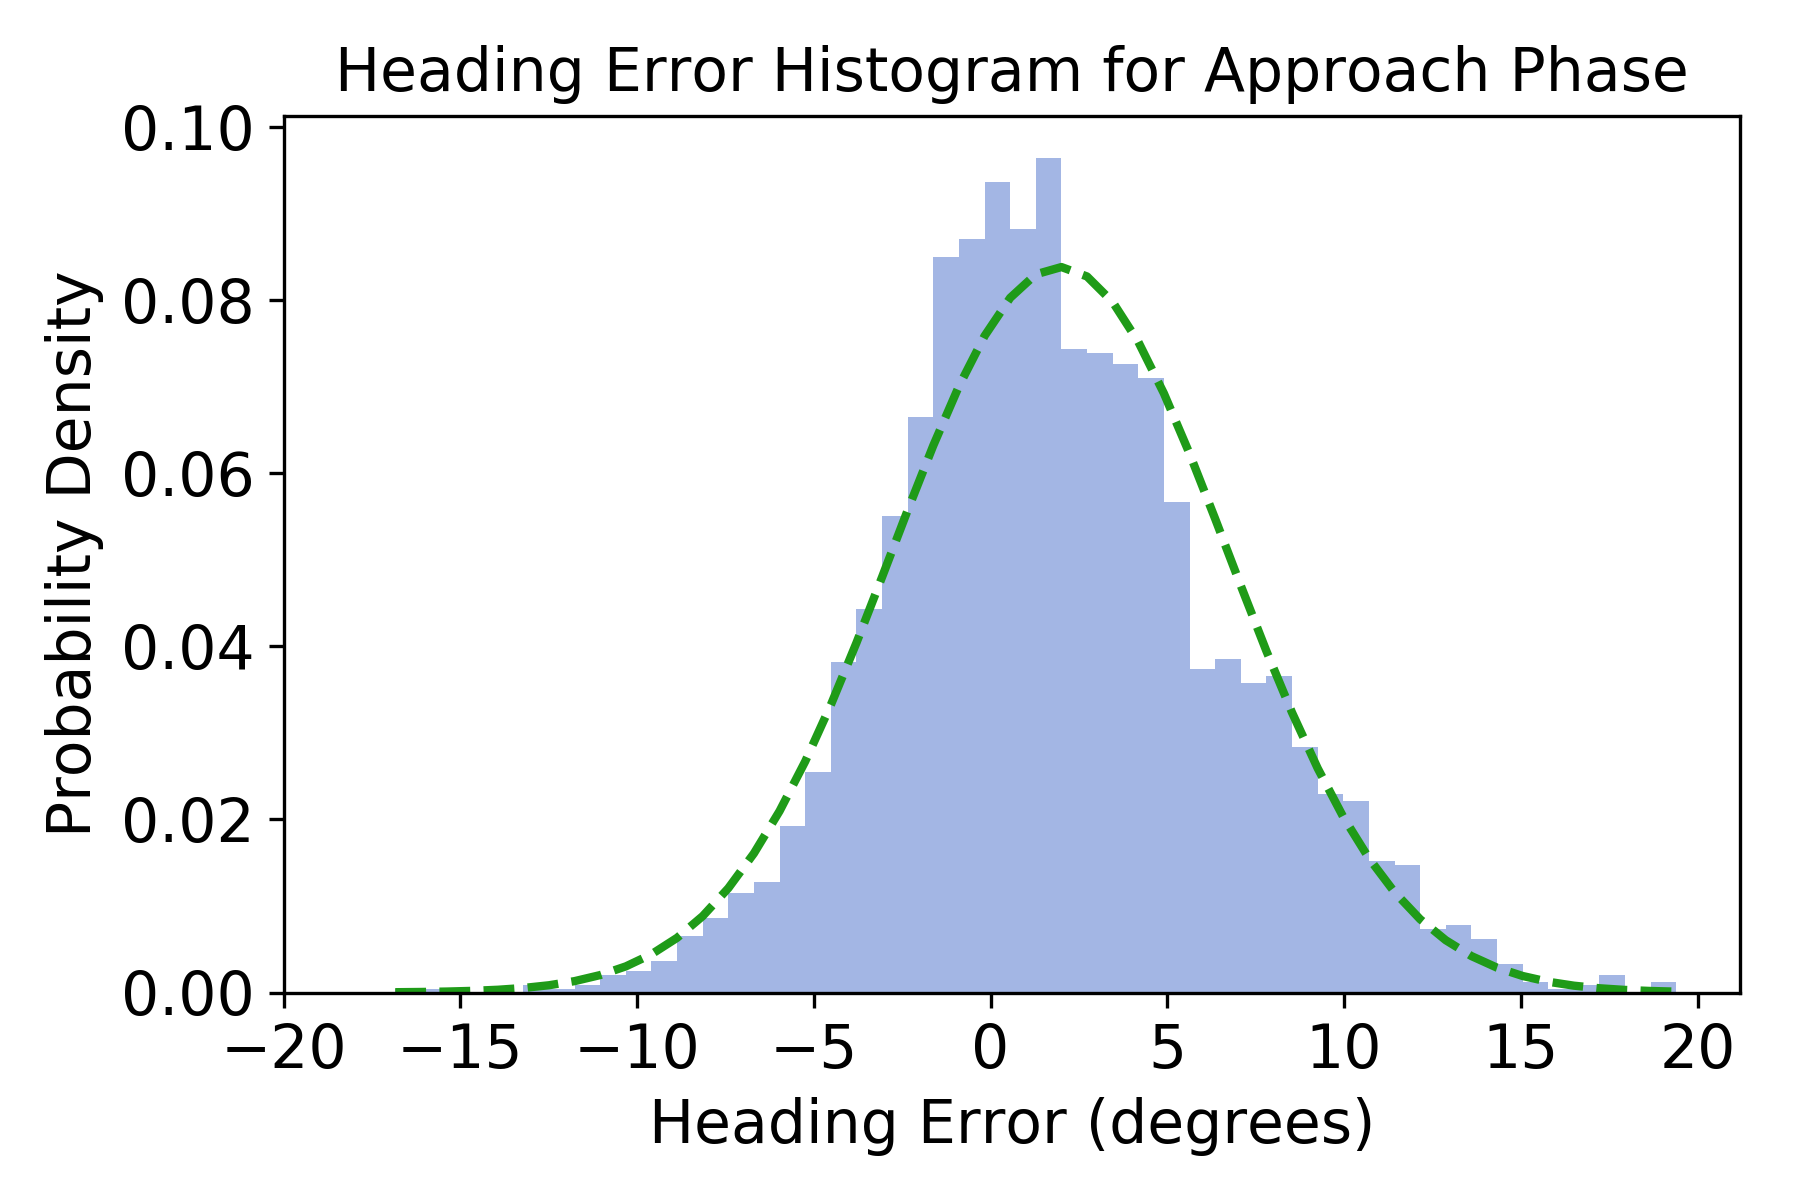
\includegraphics[width=0.45\linewidth]{orig_heading_hist}
        }%
        \caption{Histograms showing the frequencies of values for each parameter during all approach phases.  Each graph also has a dotted best-fit line to show how close the frequencies adhere to a normal distribution.}
        \label{fig:approach_histograms}
    \end{figure}
    
    
    	%----------
        % FINAL TURN
        %----------
        \paragraph{Final Turn}
        
        	Out of the 380 detected approaches; 262 (68.95\%) had a final turn subphase, 76 (20.00\%) performed a straight-in approach, and 42 (11.05\%) were not able to detect the runway and, therefore, could not detect whether a final turn was performed.  \Cref{fig:final_turn_results_ratios} depicts these ratios.  As mentioned earlier, the 42 \textit{null} runways will be drastically reduced in the future once additional airports and runways are added to the geological database.  Once the airport and runway databases are more complete, the runway error rate should become much more acceptable.
            
            \Cref{fig:final_turn_results_by_risk} gives a comparison of the number of occurrences for each turn error type and Risk Level classification.  This graph is displaying the subset of 262 detected final turn subphases found in \Cref{fig:final_turn_results_ratios}.  The figure shows that 76.34\% of the final turns resulted in an undershoot and a large proportion (45.42\%) resulted in a Risk Level 2 undershoot.  Those statistics are definitely interesting and are an example of an anomaly that is worth looking into by an aviation expert.  One explanation could be that there is frequently a strong wind component against the aircraft, which could cause the numerous undershoots.  Further analysis such as this could be performed as a future work since wind and other meteorological factors were not taken into consideration in the analyses within this research.
            
            \begin{figure}
            	\centering
                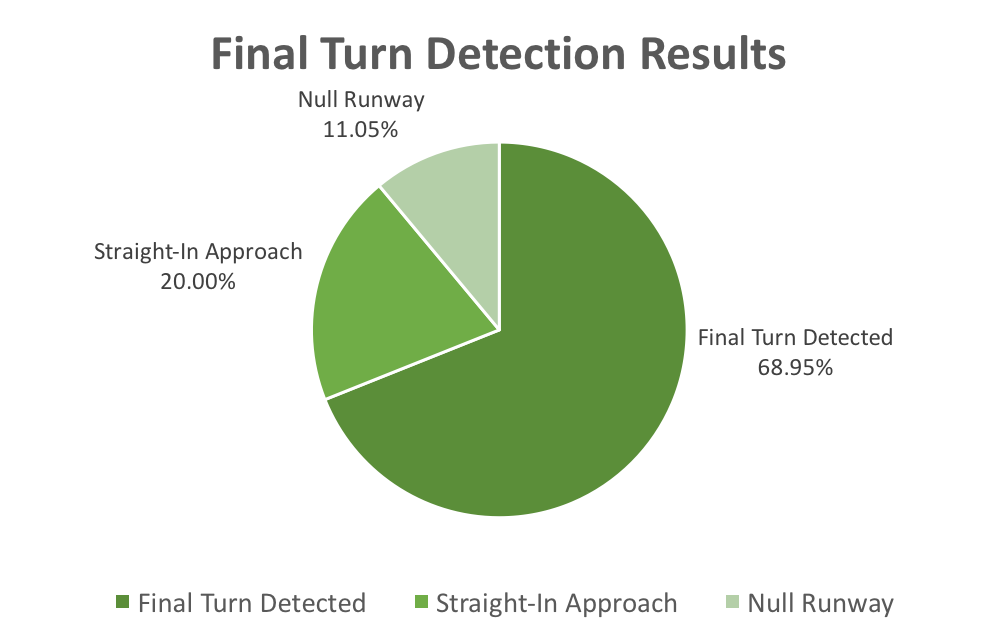
\includegraphics[width=0.75\linewidth]{final_turn_detection_results}
                \caption{Pie chart showing the results from the final turn detection algorithm.}
                \label{fig:final_turn_results_ratios}
            \end{figure}
            
            \begin{figure}
            	\centering
                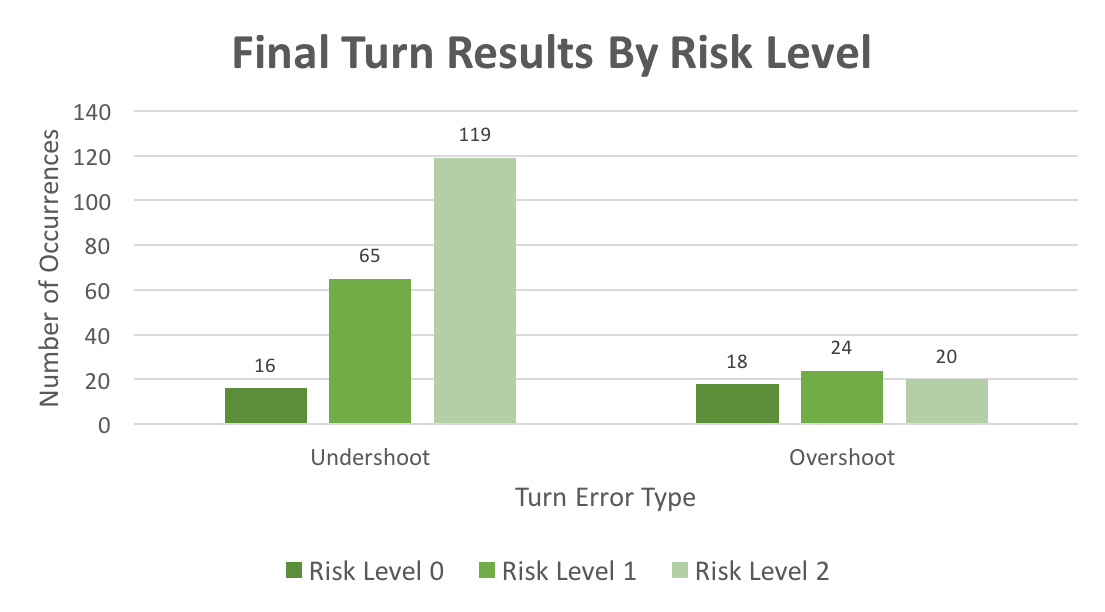
\includegraphics[width=0.95\linewidth]{final_turn_results_by_risk}
                \caption{Frequency of the occurrences of each turn error type for Risk Levels 0, 1, and 2.}
                \label{fig:final_turn_results_by_risk}
            \end{figure}


%----------------------------------------
% GRADING METRICS: DEFINE FROM PARAMETER FREQUENCIES
%----------------------------------------
\subsection{Grading Metrics:  Defined From Parameter Frequencies}

	As mentioned in \Cref{sec:methodology}, the goal for creating the Risk Level metrics is to use statistical results from the approach quality analysis to determine reasonable values that still adhere to the published stable value ranges.  \Cref{subfig:approach_ias_hist,subfig:approach_vsi_hist,subfig:approach_cross_track_hist,subfig:approach_heading_hist} above contain normalized histograms showing the probability density for the parameter values.  These graphs were analyzed by an aviation statistics expert from UND in order to create a safe range (Risk Level 0), a moderate risk range (Risk Level 1), and a high risk range (Risk Level 2) for each parameter of concern.  These graphs will be re-used in the following Sections, but will have additional information showing the value ranges that were created.  The Risk Level 1 values will be a yellow dotted line, while the Risk Level 2 values will be a red dotted line.  A summary of the defined grading metrics can be seen in \Cref{tab:metrics_values} at the end of this Section.
    
    	
    %----------
    % IAS
    %----------
    \subsubsection{Indicated Airspeed Between 55 and 75 knots}
    
          The indicated airspeed values had a mean of 64.401 knots and a standard deviation of 4.535 knots.  The aviation expert stated that the UND standardization manual~\cite{und_flight_manual} has a strict safe range of 61 -0/+5 knots, and thus anything less than 61 knots should be automatically classified as a Risk Level 2.  He advised the higher Risk Level 1 should begin with any value greater than 66 knots due to the same rule.  Lastly, he advised setting the higher Risk Level 2 at 71 knots in order to use the consistent 5 knots increment, which is also relatively close to one standard deviation.  As is shown in \Cref{fig:revised_ias_hist}, the graph is slightly skewed to the right following the -0/+5 knots rule, which is more lenient towards faster speeds than slower speeds.

		\begin{figure}
			\centering
            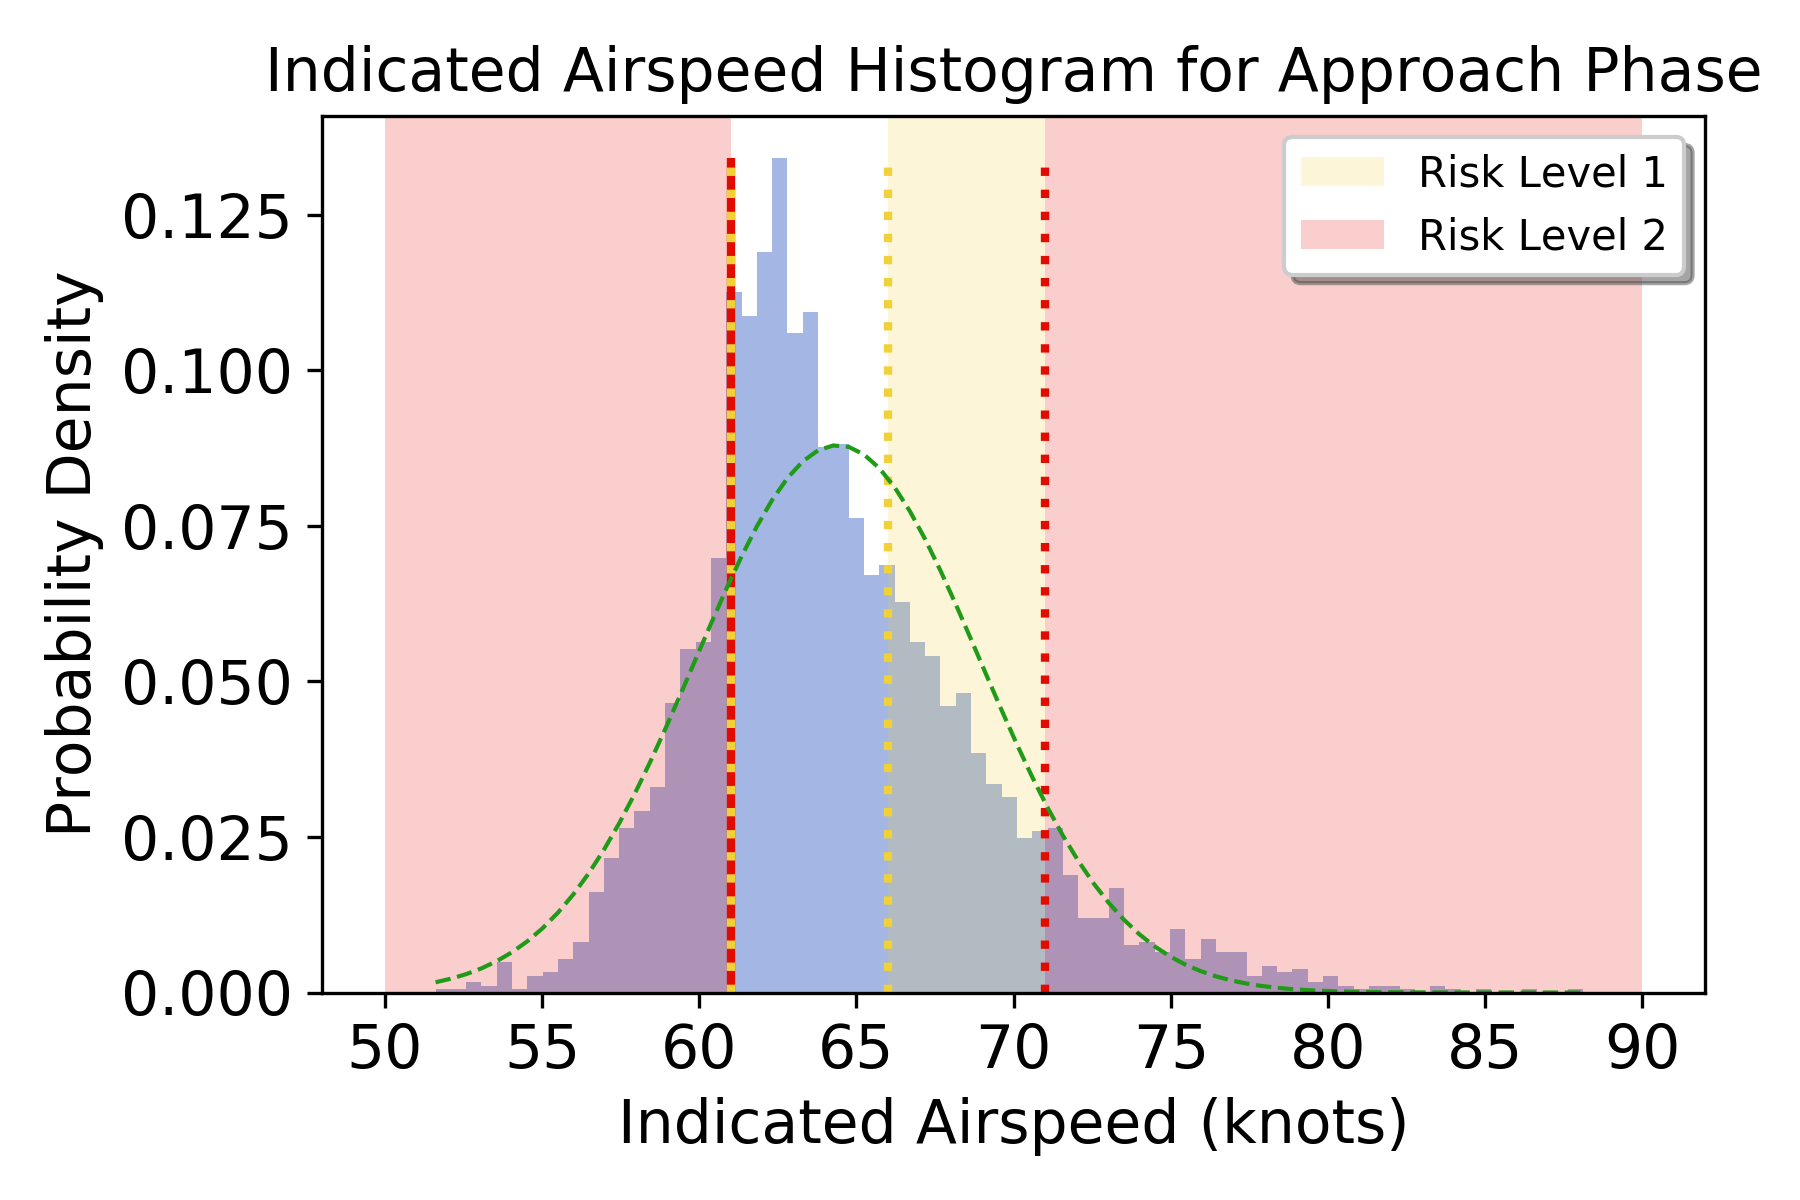
\includegraphics[width=\linewidth]{revised_ias_hist}
            \caption{Histogram for indicated airspeed ($\mu = 64.401, \sigma = 4.535$).  The safe range is between 61 and 66 knots.  The aviation expert stated that 61 knots is a hard limit according to the Cessna 172S manual~\cite{und_poh}, thus any airspeed less than 61 knots is automatically classified as a Risk Level 2.  This means there is not a lower Risk Level 1.  The higher Risk Level 1 range is between 66 and 71 knots, and the Risk Level 2 is anything greater than 71 knots.}
            \label{fig:revised_ias_hist}
		\end{figure}



    %----------
    % VSI
    %----------
    \subsubsection{Vertical Speed Indicated Greater Than -1000 ft/min}
    
    	The vertical speed indicated values had a mean of -364.528 ft/min and a standard deviation of 181.210 ft/min.  Although the UND standardization manual states that a vertical speed greater than -1000 ft/min should be achieved for a stabilized approach, the aviation expert stated that a safe range of -800 to -500 ft/min is typically suggested instead of the wide range provided in the manual.  The lower Risk Level 1 is any value that is less than -800 ft/min, and the lower Risk Level 2 is any value less than -1000 ft/min in order to adhere to the stable limit given in the manual.  The higher Risk Level 1 is any value greater than -500 ft/min, and the higher Risk Level 2 is any value greater than -250 ft/min.  These higher limits were chosen because if the aircraft is descending at 250 ft/min, it will typically result in an unsafe and shallow glide slope.  \Cref{fig:revised_vsi_hist} shows these limits and shows that the values are slightly skewed to the left, which corresponds to the risk limits that we've set.

		\begin{figure}[t]
			\centering
            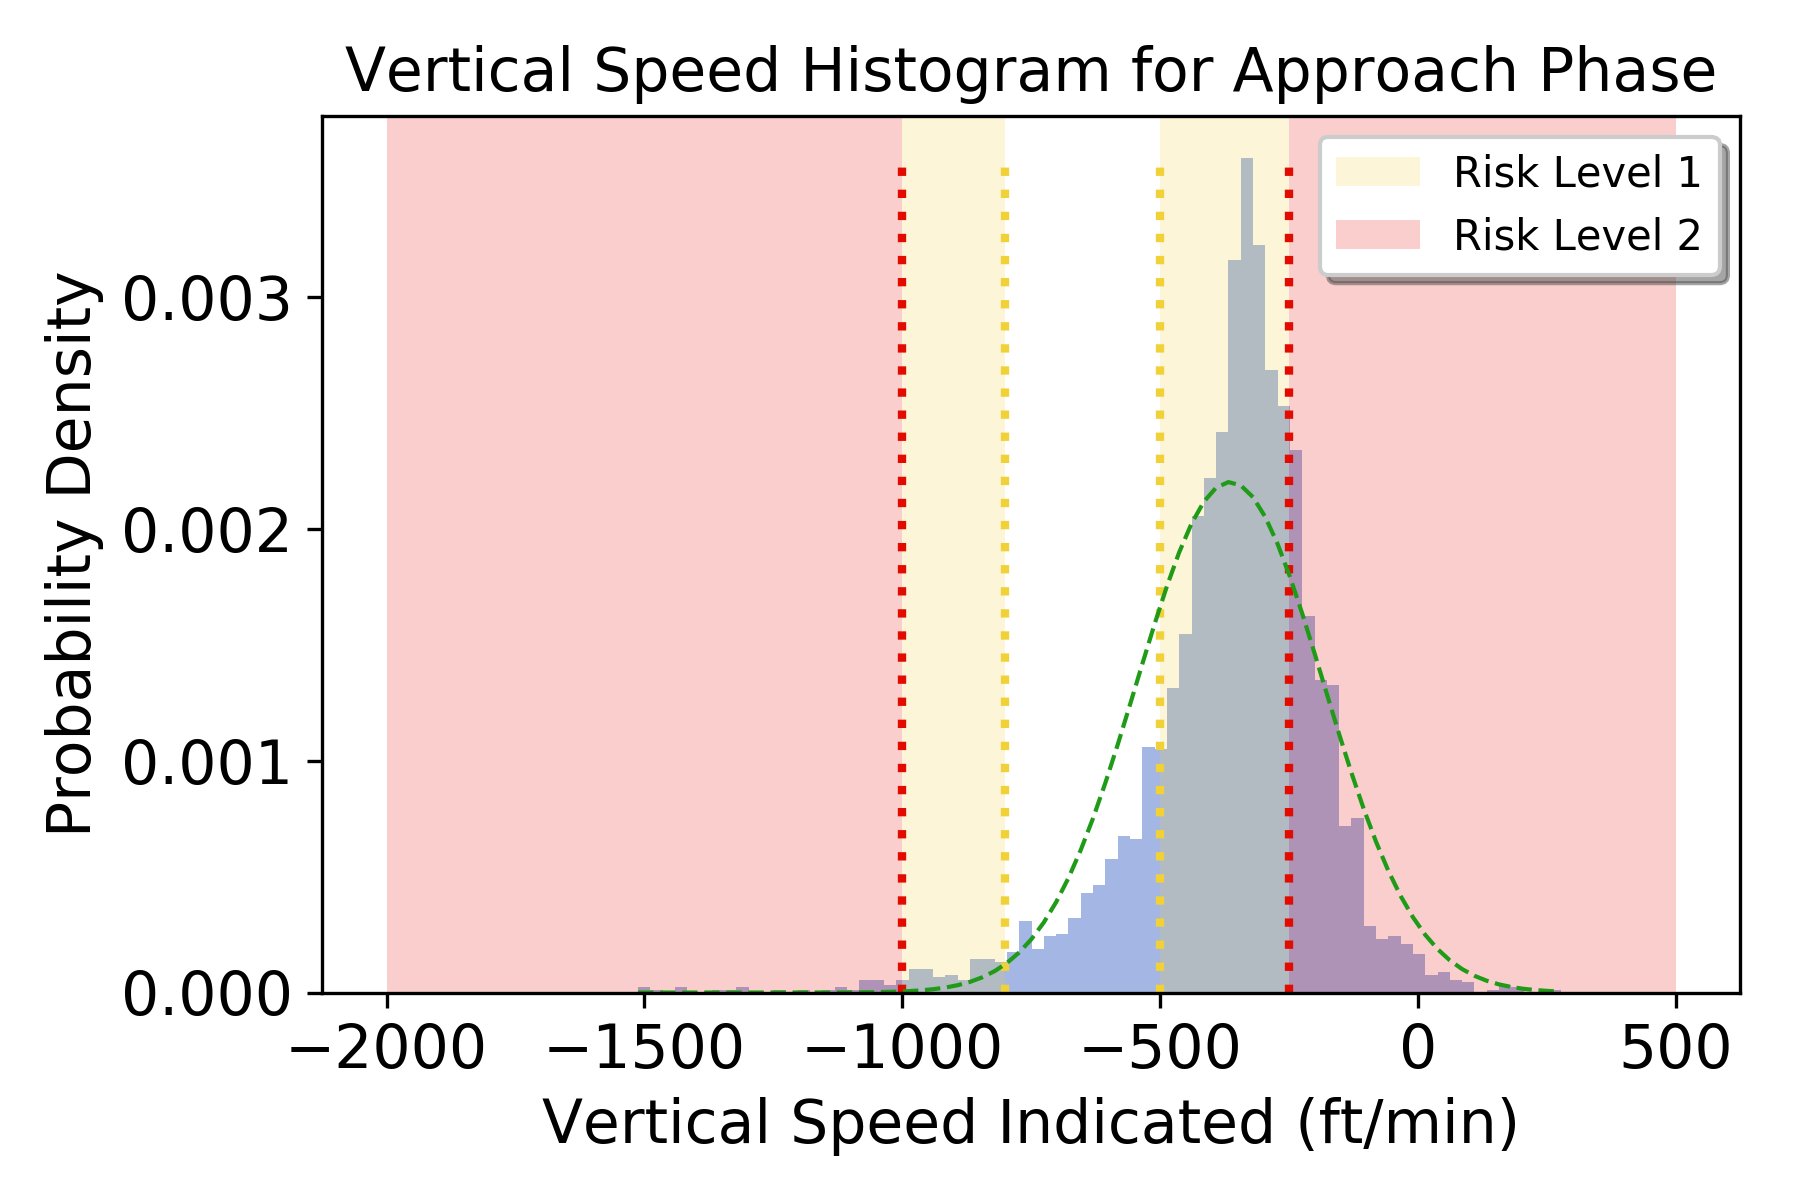
\includegraphics[width=\linewidth]{revised_vsi_hist}
            \caption{Histogram for vertical speed indicated ($\mu = -364.528, \sigma = 181.210$).  The safe range is between -800 and -500 ft/min.  The lower Risk Level 1 range is between -1000 and -800 ft/min, and the Risk Level 2 is anything less than -1000 ft/min.  The higher Risk Level 1 range is between -500 and -250 ft/min, and the Risk Level 2 is anything greater than -250 ft/min.}
            \label{fig:revised_vsi_hist}
		\end{figure}



    %----------
    % CROSS TRACK ERROR
    %----------
    \subsubsection{Absolute Cross Track Error Less Than 50 ft}
    
    	The cross track error values had a mean of -4.542 feet and a standard deviation of 15.499 feet.  \Cref{fig:revised_cross_track_hist} displays the histogram for these values and it can be seen that the graph is relatively normal with a slight skew to the left.  The aviation expert stated that a deviation in cross track error is not as risky as a deviation in airspeed or vertical speed.  Thus, a wider safe range was defined as -40 feet to 40 feet, which is about where the tails wane on both sides.  Consequently, the lower and higher Risk Level 1 ranges are -50 feet to -40 feet and 40 feet to 50 feet, respectively.  The lower and higher Risk Level 2 values are then -50 feet and 50 feet, respectively, in order to correspond with the original stable limits that were used.
        
		\begin{figure}[t]
			\centering
            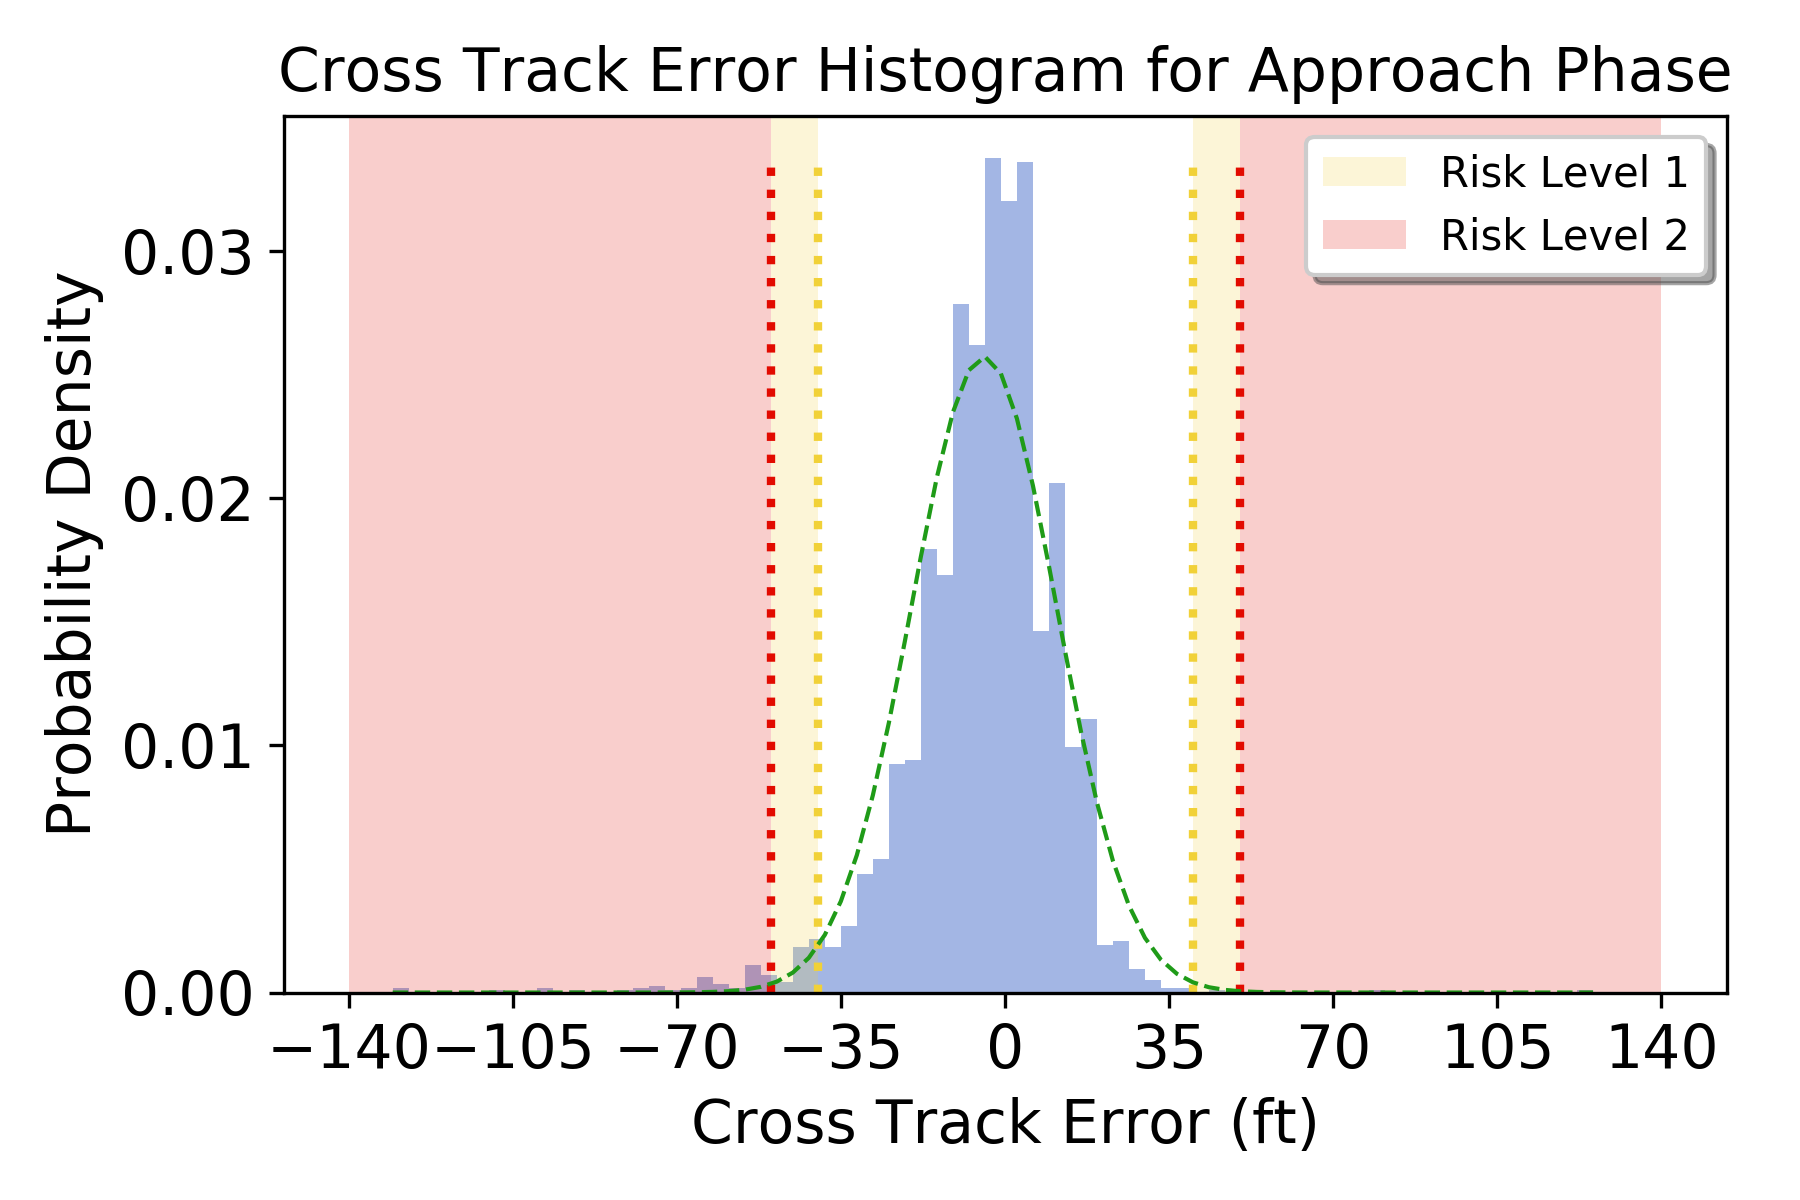
\includegraphics[width=\linewidth]{revised_cross_track_hist}
            \caption{Histogram for cross track error ($\mu = -4.542, \sigma = 15.499$).  The safe range is between -40 and 40 ft.  The lower Risk Level 1 range is between -50 and -40 ft, and the Risk Level 2 is anything less than -50 ft.  The higher Risk Level 1 range is between 40 and 50 ft, and the Risk Level 2 is anything greater than 50 ft.}
            \label{fig:revised_cross_track_hist}
		\end{figure}



    %----------
    % HEADING ERROR
    %----------
    \subsubsection{Absolute Heading Error Less Than 10 degrees}
    
    	The heading error values had a mean of $1.958^\circ$ and a standard deviation of $4.761^\circ$.  Similar to cross track error, the aviation expert stated that heading error is not as risky as error in the other parameters.  He also mentioned that heading error is slightly more difficult to judge without knowing the wind component on the aircraft since the pilot may have to purposely direct the aircraft several degrees off-center in order to counteract the push of the wind.  Both of these facts means that the safe range for heading error will contain a majority of values.  With that said, the expert advised using a safe range of $-15^\circ$ to $15^\circ$.  The lower and higher Risk Level 1 ranges are from $-20^\circ$ to $-15^\circ$ and $15^\circ$ to $20^\circ$, respectively.  Consequently, the lower and higher Risk Level 2 values are $-20^\circ$ and $20^\circ$, respectively.  The histogram for heading error, as shown in \Cref{fig:revised_heading_hist}, appears to best fit a normal distribution.
        
        \begin{figure}
			\centering
            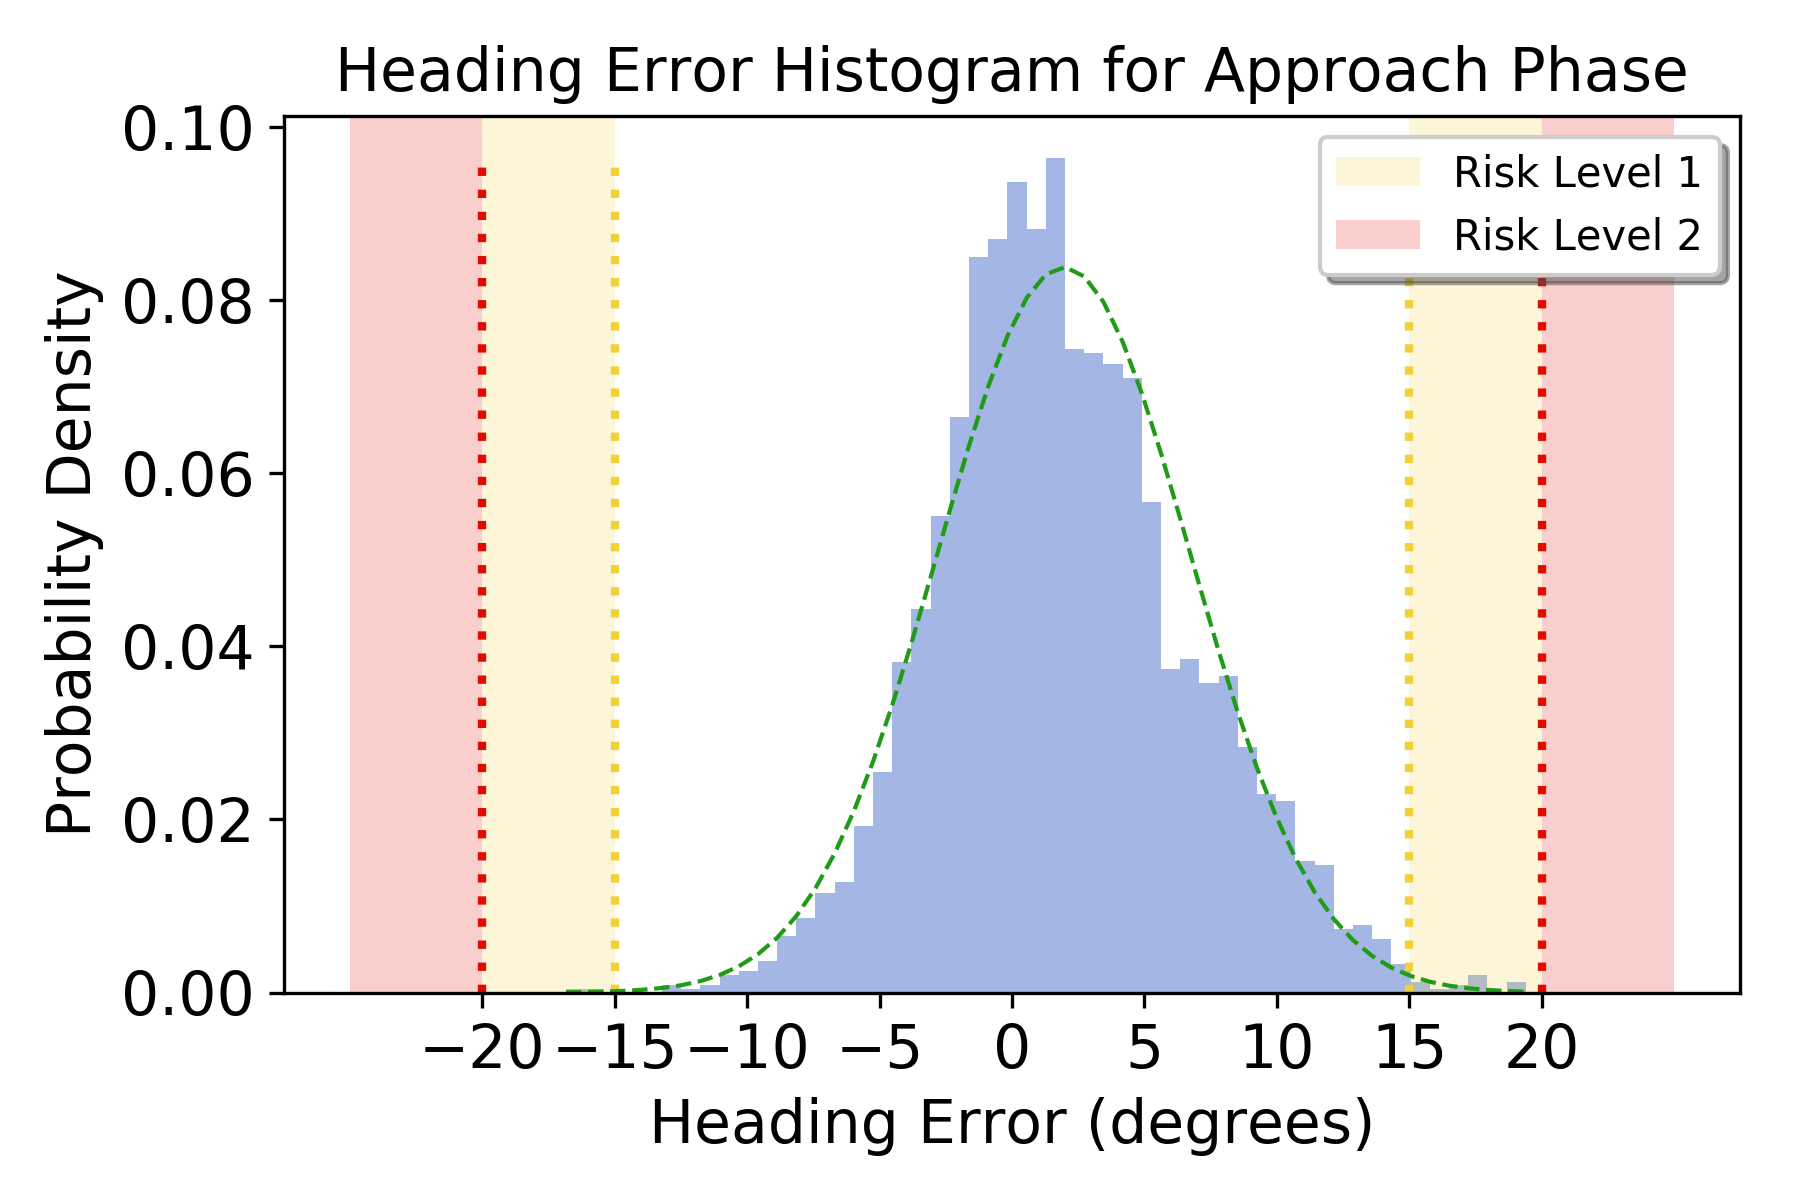
\includegraphics[width=\linewidth]{revised_heading_hist}
            \caption{Histogram for heading error ($\mu = 1.958, \sigma = 4.761$).  The safe range is between -15 and 15 degrees.  The lower Risk Level 1 range is between -20 and -15 degrees, and the Risk Level 2 is anything less than -20 degrees.  The higher Risk Level 1 is between 15 and 20 degrees, and the Risk Level 2 is anything greater than 20 degrees.}
            \label{fig:revised_heading_hist}
		\end{figure}
        
        
        
        \begin{table}
            \centering
            \caption{\small{Defined Risk Levels during approach for a Cessna C172S}} \label{tab:metrics_values}
            \vspace{3pt}
            \begin{tabular}{@{} l l | r r @{}}
                \hline\noalign{\smallskip}
                \multicolumn{2}{c|}{\bfseries Event} & \bfseries Risk Level 1 & \bfseries Risk Level 2 \\
                \noalign{\smallskip}
                \hline
                \noalign{\smallskip}
                
                \multirow{2}{*}{Indicated airspeed} & low  & N.A.     & 61 knots \\
                                                    & high & 66 knots & 71 knots \\ 
                \hline
                \multirow{2}{*}{Vertical speed} & low  & -800 ft/min & -1000 ft/min \\
                                                & high & -500 ft/min & -250 ft/min \\
                \hline
                \multirow{2}{*}{Cross track error} & low  & -40 ft & -50 ft \\
                                                   & high & 40 ft  & 50 ft \\
                \hline
                \multirow{2}{*}{Heading error} & low  & $-15^\circ$ & $-20^\circ$ \\
                                               & high & $15^\circ$  & $20^\circ$ \\
                \hline
            \end{tabular}
        \end{table}
            

%----------------------------------------
% GRADING METRICS: RESULTS
%----------------------------------------
\subsection{Grading Metrics:  Experiment Results}
	
	Using the metrics defined in the previous Section, the sample set of flights was re-analyzed in order to determine the risk levels of each parameter for every approach.  This was done by taking all the values for a parameter during the approach phase, averaging the values, and determining what risk level range the average fell within.  \Cref{fig:metric_parameter_results} shows the frequency of each parameter grouped by risk level as a result of the re-analysis.  From the graph we can see some trends such as the frequency of Risk Level 2 vertical speeds being abnormally higher than the frequency of Risk Level 1.  This may mean that the sample set contained an abnormal number of approaches with too low or too high rate of descent.  We can also see that Risk Level 0 made up a majority of occurrences for heading and cross track, which follows the fact that these parameters are typically less risky as mentioned in their previous corresponding Subsections.
	
	\begin{figure}
		\centering
		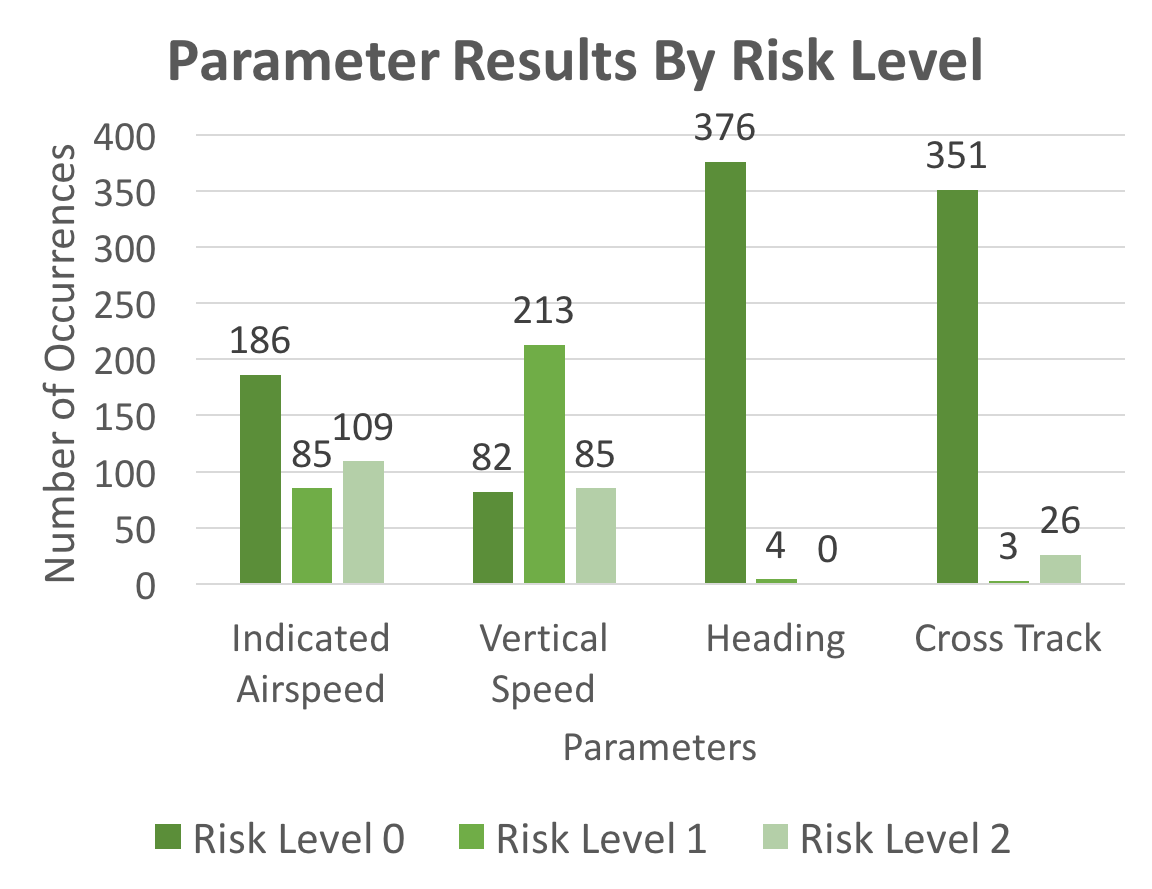
\includegraphics[width=\linewidth]{metric_parameter_results}
		\caption{Frequency of the occurrences of each parameter for Risk Levels 0, 1, and 2 using the newly defined risk level values.}
		\label{fig:metric_parameter_results}
	\end{figure}
	
	
	With regard to grading the approaches, the total number of deductions is calculated by summing the risk levels across all parameters as well as the final turn risk level.  For example; if during an approach the aircraft achieved a Risk Level 2 in indicated airspeed, a Risk Level 1 in vertical speed, a Risk Level 1 undershoot for the final turn, and a Risk Level 0 for all other parameters; the total number of deductions is 4\footnote{$2\,\text{(IAS)} + 1\,\text{(VSI)} + 1\,\text{(final turn)} + 0\,\text{(cross track)} + 0\,\text{(heading)} = 4\,\text{deductions}$}.  Additionally, if the aircraft was unstable during the approach and the pilot did not perform a go-around, an additional one deduction is added to the total.  The total number of deductions is then multiplied by a penalty constant.  The penalty points are subtracted from a total of 100 points in order to obtain the final grade for the approach.  In this research, a value of 4 points is used as the penalty per deduction.  This value was chosen because there is a possibility of accruing 11 total deductions\footnote{2 risk levels * 4 parameters + 2 final turn risk levels + 1 for unstable w/o go-around = 11}, which would create a total of 44 penalty points.  Thus, the worst possible grade to receive would be 56 points\footnote{If using a 90-80-70-60\% grading scale, this would then correspond to an F.}.  \Cref{fig:scores_hist} gives a histogram of the grades calculated for the sample set of 100 flights used during the experiments.  For the grades of the sample set, the mean was 87.168 points and a standard deviation of 7.260 points.  As the figure shows, the histogram reasonably fits a normal distribution, but slightly skewed to the right.  These results have given us good confidence that the grading system will replicate the grading structure already used in Universities that students are already accustomed to.
	
	\begin{figure}
		\centering
		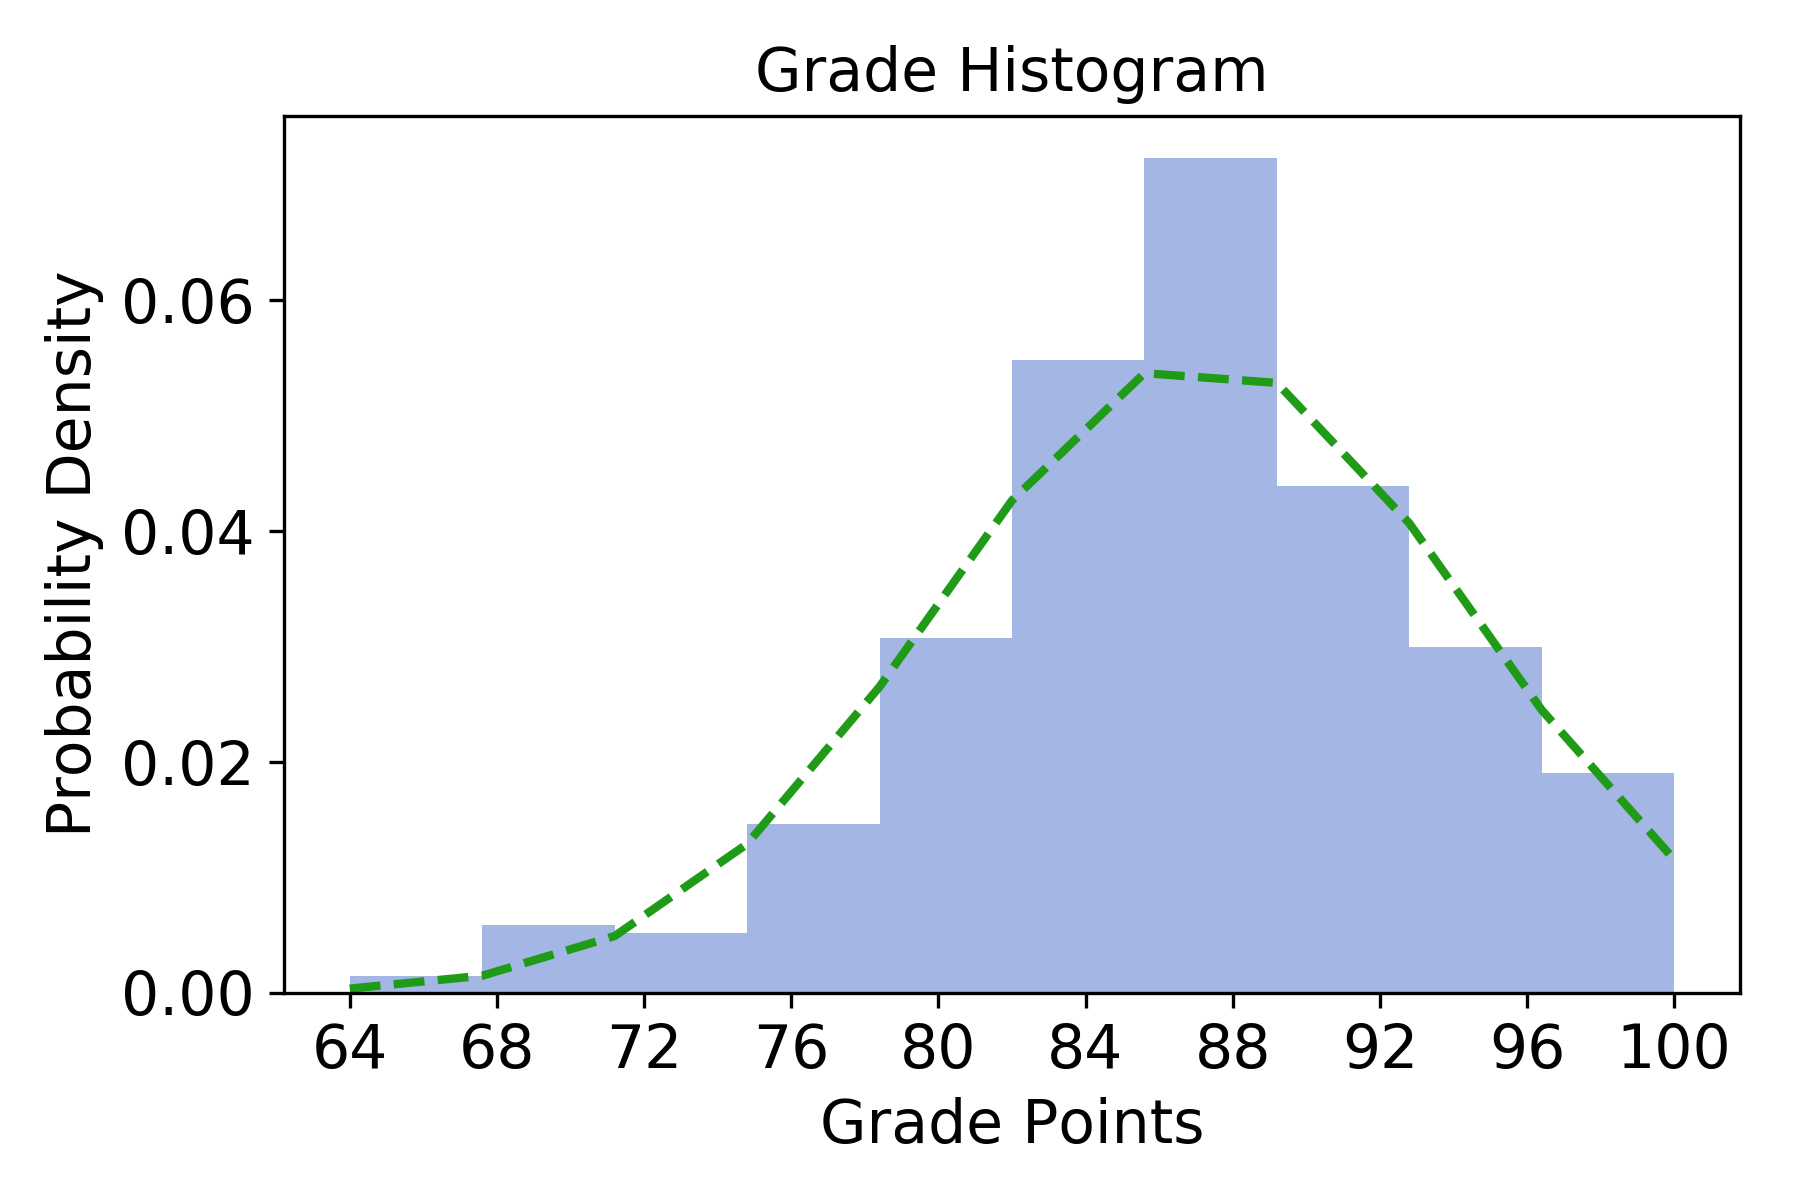
\includegraphics[width=\linewidth]{orig_scores_hist}
		\caption{Histogram showing the results of grading approach phases.  Each grade is calculated by totaling the risk levels across all parameters then multiplying the sum by a penalty amount per deduction.}
		\label{fig:scores_hist}
	\end{figure}
        

%----------------------------------------
% PERFORMANCE
%----------------------------------------
\subsection{Performance}

	A secondary aspect of this research is to minimize the execution time so the analysis only adds a minimal amount of time to a flight being imported into the NGAFID system.  The results of the benchmarking tests showed that the linearly executing application ran for an average of 127.109 seconds over the 100 randomly tested flights.  On the other hand, the parallel application ran for an average of 56.935 seconds over the same flights.  This means the average per-flight execution times for the linear and parallel applications were 1.271 and 0.569 seconds, respectively.  As a result, the parallelized application had a 2.23x speedup, which is fairly significant.  A summary of the benchmarking tests and other relevant statistics are given in \Cref{tab:performance_results}.
    
    As further evidence, the parallel application was tested on a larger subset of flights to see if the average execution time remained stable, in which it was tested on 5,923 flights.  For this test, the parallel application was able to analyze the data and insert all the results into the database in 2,709.577 seconds.  This gives a per-flight execution time of 0.457 seconds, which is slightly less than the average for 100 flights.  The reasoning behind this can most likely be attributed to the fact that spinning up the sub-processes creates a substantial overhead.  Thus, the longer the application is able to execute, the greater performance gain will be received.  This will, of course, start to show diminishing returns as with any other parallel computing application.
    
    
    \begin{table}[tb]
    	\centering
        \caption{\small{Performance of Linear v. Parallel Execution Times}} \label{tab:performance_results}
        \vspace{3pt}
        \begin{tabular}{@{} >{\centering\arraybackslash} m{.23\linewidth} S[table-format=3.3] S[table-format=2.3] @{}}
            \hline\noalign{\smallskip}
            \bfseries Run \# & \bfseries Linear (sec) & \bfseries Parallel (sec) \\
            \noalign{\smallskip}
            \hline
            \noalign{\smallskip}
             1 & 128.275 & 56.726 \\ \hline
             2 & 130.441 & 56.086 \\ \hline
             3 & 127.878 & 61.263 \\ \hline
             4 & 121.923 & 55.787 \\ \hline
             5 & 126.418 & 57.964 \\ \hline
             6 & 125.425 & 55.753 \\ \hline
             7 & 126.123 & 57.945 \\ \hline
             8 & 128.949 & 55.830 \\ \hline
             9 & 128.161 & 55.497 \\ \hline
            10 & 127.494 & 56.496 \\ \hline
            \hline
            \bfseries Average           & 127.109 & 56.935 \\ \hline
            \bfseries Latency / flight  &   1.271 &  0.569 \\ \hline
            \bfseries Speedup           &         &  2.23x \\ \hline
        \end{tabular}
    \end{table}
    
    
    
    
%% !TEX root =  ../main.tex

\section{Conclusion} \label{sec:conclusion}
	
	This article presented the \toolname, an application designed to augment the existing features of the National General Aviation Flight Information Database (NGAFID).  The purpose of creating the application is to provide student pilots and Certified Flight Instructors (CFI) with metrics-based feedback on flight performance during critical phases of flight.  The desired effects of this are \textit{(i)} target different student learning techniques, \textit{(ii)} improve the efficiency and reduce the cost of flight training, and \textit{(iii)} reduce General Aviation (GA) accident and fatality rates since GA is the most dangerous branch of Civil Aviation.  Additionally, the application is currently geared towards analyzing the approach and landing phases as these phases of flight are where a majority of pilot-related accidents occur.
	
	Using flight data recorder (FDR) data generated by a Garmin G1000 from Cessna C172S aircraft; the application can detect safety exceedances for indicated airspeed, vertical speed, cross track, and heading during the approach phase as well as classify the result of each approach as a full-stop landing, touch-and-go landing, or a go-around during the landing phase.  For the event-driven approach to successfully characterize the safety of an approach, the safety exceedance definitions needed to be internally consistent (\ie, the parameter limits need to correspond to the same level of risk to the pilot).  In this research, the safety exceedances were re-defined in a way that makes them more consistent by an aviation statistics expert who used the distributions of parameter values found during the initial experiments.  These new definitions were then used in the newly created grading system for the purpose of scoring the pilot's flight performance based on any exceedances found during the approach analysis stage.
	
	Several new web tools were created which were integrated into the NGAFID.  These tools include interfaces for \textit{(i)} displaying histograms of the aggregated parameter values during approach phases within a chosen time-frame, \textit{(ii)} visualizing final turn phases for a single flight or an aggregate of flights at a chosen runway, and \textit{(iii)} displaying a histogram of self-defined glide path angles within a chosen time-frame at a given runway.
	
	The performance of the application run in parallel averaged 0.569 seconds per flight for the sample set of 100 flights, while an analysis of 5,923 flights averaged 0.457 seconds per flight.  This shows that the application has a reasonably short run-time and can be used practically in the NGAFID's production environment.


\subsection{Future Work} \label{sec:future_work}

	This research has provided many avenues for further work and refinement.  First, the greatest constraint on the accuracy of the application is the accuracy of the instrument recording the flight data, whether that be a traditional FDR or a smartphone.  This means that if data is recorded inaccurately, it is useless to the application and cannot be recovered.  For example, in several of the sample flights, the first 10 to 20 rows of data can have missing and/or spurious values due to the aircraft's sensors calibrating after first starting the FDR.  Invalid data rows can occur during the middle of a flight as well; not only when the FDR is initially turned on.  Thus, further work into filtering, sanitizing, or normalizing faulty data would be very beneficial.
	
	Second, it would be beneficial to make the algorithms more modular in order to analyze data from different sources.  For example, a source with a limited number of parameters it records, such as a smartphone, or a completely different FDR brand.
	
	Third, this research focused solely on the analysis of flight performance and generation of metrics describing the performance, thus further work in the area of UI/UX would be a great next step.  This future research would ideally focus on the most effective way to display the metrics to the user and improve upon the user-friendliness of the web interfaces introduced in this work.
	
	Lastly, the algorithms introduced in this research can be extended to analyze other phases of flight (\eg, takeoff, climb, cruise, etc.).  This means that new risk level values would need to be defined as well to fit the data found in the new analyses.
    
    Once the \toolname\ is fully integrated into the NGAFID, it will provide even more possibilities for data visualization and be easily accessible for both novice and experienced pilots.  This will allow pilots on an individual or organizational level to become more aware of bad flight habits so they may correct them in future flights and help make General Aviation safer.


%----------------------------------------------------------------------------------------
%	REFERENCES
%----------------------------------------------------------------------------------------

\section*{References}
\bibliographystyle{aiaa}
\bibliography{bibliography}

%\section*{References}
%\begin{thebibliography}{}
%\bibitem{1} Vatistas, G. H., Lin, S., and Kwok, C. K., ``Reverse Flow Radius in Vortex Chambers,'' \textit{AIAA Journal}, Vol. 24, No. 11, 1986, pp. 1872, 1873. doi: 10.2514/3.13046
%\bibitem{2} Dornheim, M. A., ``Planetary Flight Surge Faces Budget Realities,'' \textit{Aviation Week and Space Technology}, Vol. 145, No. 24, 9 Dec. 1996, pp. 44--46.
%\bibitem{3} Terster, W., ``NASA Considers Switch to Delta 2,'' \textit{Space News}, Vol. 8, No. 2, 13--19 Jan. 1997, pp. 1, 18.
%\bibitem{4} Peyret, R., and Taylor, T. D., \textit{Computational Methods in Fluid Flow}, 2$^{{\rm nd}}$ ed., Springer-Verlag, New York, 1983, Chaps. 7, 14.
%\bibitem{5} Oates, G. C. (ed.), \textit{Aerothermodynamics of Gas Turbine and Rocket Propulsion}, AIAA Education Series, AIAA, New York, 1984, pp. 19, 136.
%\bibitem{6} Volpe, R., ``Techniques for Collision Prevention, Impact Stability, and Force Control by Space Manipulators,'' \textit{Teleoperation and Robotics in Space}, edited by S. B. Skaar and C. F. Ruoff, Progress in Astronautics and Aeronautics, AIAA, Washington, DC, 1994, pp. 175--212.
%\bibitem{7} Thompson, C. M., ``Spacecraft Thermal Control, Design, and Operation,'' \textit{AIAA Guidance, Navigation, and Control Conference}, CP849, Vol. 1, AIAA, Washington, DC, 1989, pp. 103--115
%\bibitem{8} Chi, Y. (ed.), \textit{Fluid Mechanics Proceedings}, NASA SP-255, 1993.
%\bibitem{9} Morris, J. D., ``Convective Heat Transfer in Radially Rotating Ducts,'' \textit{Proceedings of the Annual Heat Transfer Conference}, edited by B. Corbell, Vol. 1, Inst. of Mechanical Engineering, New York, 1992, pp. 227--234.
%\bibitem{10} Chapman, G. T., and Tobak, M., ``Nonlinear Problems in Flight Dynamics,'' NASA TM-85940, 1984.
%\bibitem{11} Steger, J. L., Jr., Nietubicz, C. J., and Heavey, J. E., ``A General Curvilinear Grid Generation Program for Projectile Configurations,'' U.S. Army Ballistic Research Lab., Rept. ARBRL-MR03142, Aberdeen Proving Ground, MD, Oct. 1981.
%\bibitem{12} Tseng, K., ``Nonlinear Green's Function Method for Transonic Potential Flow,'' Ph.D. Dissertation, Aeronautics and Astronautics Dept., Boston Univ., Cambridge, MA, 1983.
%\bibitem{13} Richard, J. C., and Fralick, G. C., ``Use of Drag Probe in Supersonic Flow,'' \textit{AIAA Meeting Papers on Disc} [CD-ROM], Vol. 1, No. 2, AIAA, Reston, VA, 1996.
%\bibitem{14} Atkins, C. P., and Scantelbury, J. D., ``The Activity Coefficient of Sodium Chloride in a Simulated Pore Solution Environment,'' \textit{Journal of Corrosion Science and Engineering} [online journal], Vol. 1, No. 1, Paper 2, URL: \url{http://www.cp/umist.ac.uk/JCSE/vol1/vol1.html} [cited 13 April 1998].
%\bibitem{15} Vickers, A., ``10-110 mm/hr Hypodermic Gravity Design A,'' \textit{Rainfall Simulation Database} [online database], URL: \url{http://www.geog.le.ac.uk/bgrg/lab.htm} [cited 15 March 1998].
%\bibitem{16} TAPP, Thermochemical and Physical Properties, Software Package, Ver. 1.0, E. S. Microware, Hamilton, OH, 1992.
%\bibitem{17} Scherrer, R., Overholster, D., and Watson, K., Lockheed Corp., Burbank, CA, U.S. Patent Application for a ``Vehicle,'' Docket No. P-01-1532, filed 11 Feb. 1979.
%\bibitem{18} Doe, J., ``Title of Paper,'' \textit{Name of Journal} (to be published).
%\bibitem{19} Doe, J., ``Title of Chapter,'' \textit{Name of Book}, edited by\ldots , Publisher's name and location (to be published).
%\bibitem{20} Doe, J., ``Title of Work,'' Name of Archive, Univ. (or organization), City, State, Year (unpublished).
%\end{thebibliography}


\end{document}
